\documentclass [fontsize=14pt, paper=a4, pagesize, DIV=calc] {scrartcl}
% \documentclass [fontsize=14pt] {scrartcl}
% \documentclass [12pt] {article}

\usepackage{ragged2e}
\justifying

\usepackage[a4paper, left=3.0cm, right=1.5cm, top=2.0cm, bottom=2.0cm, footskip=1.0cm]{geometry}
\setlength{\parindent}{1.25pt}
\usepackage{setspace}
\onehalfspacing

% graphics
\usepackage{pstool}                    % post-script editing from latex
\usepackage[dvips]{rotating,graphicx}  % use graphics 
\usepackage{float}                     % enables float options (positioning of elements)
\usepackage{soul}
\usepackage{xcolor}

\usepackage{blindtext}

% fonts
\usepackage[utf8]{inputenc}
% \usepackage[t2a]{fontenc}
% \usepackage{lmodern}                   % loads latin-modern fonts
\usepackage[T1]{fontenc}
\usepackage{mathptmx}
\usepackage{slashed}
\usepackage{color}                     % use colors in text

\usepackage{sectsty}
\allsectionsfont{\fontfamily{ptm}\bfseries}
\sectionfont{\fontsize{22}{15}\bfseries\fontfamily{ptm}\selectfont}
\subsectionfont{\fontsize{20}{15}\bfseries\fontfamily{ptm}\selectfont}


\usepackage{mathrsfs}
% links
\usepackage{hyperref}
\hypersetup{
            %backref,  % already set somewhere
            pdfpagemode=UseOutlines,
            linkcolor=[RGB]{0,51,160}, % blue,
            citecolor=[RGB]{0,51,160}, % blue,
            urlcolor=[RGB]{0,51,160}, % blue,
            % hyperfigures=true,  % already set somewhere
            colorlinks=true}

\parindent=14pt

\usepackage{euscript}	 % Шрифт Евклид
\usepackage{mathrsfs} % Красивый матшрифт
\usepackage{enumitem}  % helps to make smaller dots in enum
\usepackage{latexsym}

% other styles
\usepackage{enumitem}  % helps to make smaller dots in enum
\usepackage{latexsym}

% math
\usepackage{siunitx}                        % use si units with \si{unit} or \SI{#}{unit}
\usepackage{amsmath,amsfonts,amssymb,amsthm,mathtools} % AMS
% \usepackage{bm}                             % bold math symbols
\usepackage{gensymb}
\newcommand{\proptoinverse}{\mathrel{\mskip1mu\reflectbox{$\propto$}\mskip-1mu}}

% Define header and footer
\usepackage{lastpage}
\usepackage{fancyhdr}
\fancypagestyle{plain}{%
\fancyhf{} % clear all header and footer fields
\fancyfoot[C]{\fontfamily{cmr}\fontsize{14pt}{14pt}\selectfont\thepage} % except the center
\renewcommand{\headrulewidth}{0pt}
\renewcommand{\footrulewidth}{0pt}}
% \usepackage[a4paper,margin=1cm,footskip=0.5cm]{geometry}

% \usepackage{float}
% \restylefloat{table}

\usepackage{graphicx}
\usepackage{caption}
% \captionsetup[figure]{name=Рисунок}
% \DeclareCaptionSubType*[asbuk]{figure}
% \captionsetup[subfigure]{labelformat=}
\usepackage{subcaption}
\renewcommand\thesubfigure{\asbuk{subfigure}}
\usepackage{subfloat}


\usepackage{wrapfig}
\usepackage{tabularx}

% tables
\usepackage{multirow}       % allows multiple rows put into one
\usepackage{booktabs}       % hline extensions like \toprule \bottomrule \midrule 
\usepackage{makecell}       % multiline cells

% references
\usepackage{cite}
% \usepackage[backend=bibtex, citestyle=numeric,bibstyle=authortitle]{biblatex} %Imports biblatex package
% \addbibresource{mybib.bib} %Import the bibliography file
% \renewcommand\citeform[1]{[#1]}
\usepackage[nameinlink,capitalize]{cleveref}  % easy referencing

\usepackage[russian]{babel}
% table of contents settings
\usepackage{tocloft}
\usepackage{titlesec}
\cftsetindents{section}{0em}{2em}
% \cftsetindents{subsection}{0em}{2em}
\renewcommand\cfttoctitlefont{\hfill\Large\bfseries}
\renewcommand\cftaftertoctitle{\hfill\mbox{}}
\renewcommand{\cftsecleader}{\cftdotfill{\cftdotsep}}
\newlength{\anIndent}
\setlength{\anIndent}{\parindent}

\titleformat{\section}
  {\normalfont\Large\bfseries}{\thesection}{2\anIndent-\widthof{\thesection}}{}

\titleformat{\subsection}
  {\normalfont\large\bfseries}{\thesubsection}{3\anIndent-\widthof{\thesubsection}}{}

\titleformat{\subsubsection}
  {\normalfont\normalsize\bfseries}{\thesubsubsection}{4\anIndent-\widthof{\thesubsubsection}}{}

\newenvironment{indentedSection}[1]{%
    %Input #1: Level of indentation
    \begin{adjustwidth}{#1\anIndent+\anIndent}{}
        \hspace{\anIndent}% Indent first line
        \ignorespaces% Ignor any space at start of environment
    }{\end{adjustwidth}}

\setcounter{tocdepth}{3}

\DeclareMathOperator{\sgn}{\mathop{sgn}}
\DeclareMathOperator{\Div}{div}
\DeclareMathOperator{\Rot}{rot}
\numberwithin{equation}{section}
\DeclareMathOperator\erfc{erfc}
\DeclareOldFontCommand{\sc}{\normalfont\bfseries}{\textsc}
%


\begin{document}

% Title Page %%%%%%%%%%%%%%%%%%%%%%%%%%%%%%%%%%%%%%%%%%%%%%%%%%%%%%%%%%%%%%%%%%%%%%%%%%%%%%%% 
\pagestyle{empty}
\begin{titlepage}
\begin{center}
%\vspace*{1\baselineskip}

{\large \textbf{Министерство науки и высшего образования Российской Федерации
федеральное государственное автономное образовательное учреждение высшего образования
}}

\vspace*{1\baselineskip}

{\Large \textbf{Национальный исследовательский ядерный университет «МИФИ»}}

\vspace*{2\baselineskip}

{\Large \textbf{Кафедра №97}}

\vspace*{1\baselineskip}

{\Large \textbf{«Суперкомпьютерное моделирование в инженерно-физических процессах»}}

\vspace*{1\baselineskip}

{\Large \textbf{Дипломная работа}}

\vspace*{1\baselineskip}

{\Large  {\textbf{''Динамические характеристики\\нестационарного дебаевского слоя''}}}

\end{center}
\vspace*{2\baselineskip}
\begin{flushright}
\begin{large}
Выполнил:\\
студент группы Б21---221\\
Шатилов И. А.\\
Научный руководитель:\\
к.ф.-м.н. доцент каф.21\\
Степаненко А. А.
\end{large} 
\end{flushright}

\vspace*{2\baselineskip}
\begin{center}
Москва --- 2025
\end{center}
\end{titlepage}
\pagebreak

% Description %%%%%%%%%%%%%%%%%%%%%%%%%%%%%%%%%%%%%%%%%%%%%%%%%%%%%%%%%%%%%%%%%%%%%%%%%%%%%%%%%%%%%%%%%%%%%%%%%%%%%%%%%%%%%%%%%%%%%%%%%%%%%%
\pagestyle{plain}
\tableofcontents
\pagebreak
\section{Введение}
\qquadСоздание термоядерного реактора требует исследования тепловых нагрузок на
внутреннюю поверхность установки и моделирования движения филаментов. ПЛМ,
возникающие во всех конфигурациях установок магнитного удержания плазмы имеют
аналогичные свойства, одним из которых является резкое(время развития ПЛМ
составляет порядка $50-100$ мкс) сильное увеличение теплового
потока(\hl{сколько?}). В перспективных и некоторых существующих токамаках
наблюдается плавление материала, что в случае проплавления материала моноблока
является неприемлимым для работы токамака~\cite{gunn2017surface}. Анализ
подобных выбросов и их влияния на параметры дебаевского слоя является одной из
главных задач на пути к созданию стабильных в работе и коммерчески успешных
термоядерных установок с магнитным удержанием плазмы.

Решение задачи моделирования динамики плазмы требует определения параметров
дебаевского слоя --- граничного условия. Существующие модели, как правило, не
учитывают наличие осцилляций магнитного поля, возникающих в дебаевском слое при
прохождении филаментов по поверхности. Анализ характера изменения параметров
дебаевского слоя и осцилляций магнитного поля в филаменте позволяет предполагать
увеличение значения усреднённого теплового потока на поверхность стенки. Так же,
ввиду изменения разности потенциалов в слое(плавающего потенциала) возникает
ненулевой ток, и как следствие, ненулевое сопротивление дебаевского слоя.
\pagebreak

\section{Обозначения и сокращения}
\begin{align*}
	\theta(x) &\text{ --- функция Хевисайда}\\
	\text{ПЛМ} &\text{ --- пограничная локализованная мода}\\
	a &\text{ --- атомы}\\
	c_s &\text{ --- скорость звука в плазме}\\
	e &\text{ --- электроны}\\
	i &\text{ --- ионы}\\
	se &\text{ --- вход в дебаевский слой}\\
	te &\text{ --- термоэлектронная эмиссия}\\
	th &\text { --- тепловая скорость}\\
	trans &\text { --- параметр при смене режимов работы дебаевского слоя}\\
	s &\text{ --- поверхность плитки}\\
	V_f &\text{ --- плавающий потенциал}\\
	W &\text{ --- вольфрам}
\end{align*}
\pagebreak

\section{Цели и задачи}
\qquadЦель работы --- проведение анализа динамических характеристик нестационарного дебаевского слоя. Задачами являются:
\begin{itemize}
	\item Составление модели дебаевского слоя с учётом наличия термоэлектронной эмиссии с поверхности стенки
	\item Проведение численного моделирования параметров дебаевского слоя с использованием полученной модели и учётом теплопроводности в материале стенки
	\item Составление вывода о характере эволюции проводимости дебаевского слоя в присутствии осцилляций потенциала на входе в слой
	\item Проведение численного моделирования прохождения филамента по поверхности стенки с применением полученной модели в качестве граничного условия, сравнение с результатами 
		моделирования с использованием других моделей
	\item Составление вывода о значении тепловой нагрузки на стенку, сравнение с классическими значениями
\end{itemize}
\pagebreak
\pagebreak


\section{Литературный обзор}

Экстремальные тепловые нагрузки на материал стенок установки --- одна из
основных проблем создания будущих коммерчески эффективных термоядерных
реакторов. Для строящегося ITER в 2013 году в качество основных были
выбраны~\cite{merola2015engineering} плитки состоящие из $W$ и имеющие подложку
из $CuCrZr$~\autoref{pic::Motojime_tile}, способные выдерживать нагрузки до $4.7$ МВт$/$м$^2$. Плитки,
используемые в диверторах испытывают гораздо большие тепловые нагрузки и
способны выдерживать до $20$ МВт$/$м$^2$~\cite{motojima2015iter}.
Несогласованная плитка может подвергаться нагрузкам до 15---60 раз
большим~\cite{moritz2023thermionic}. 

\begin{figure}[H]
	\centering
	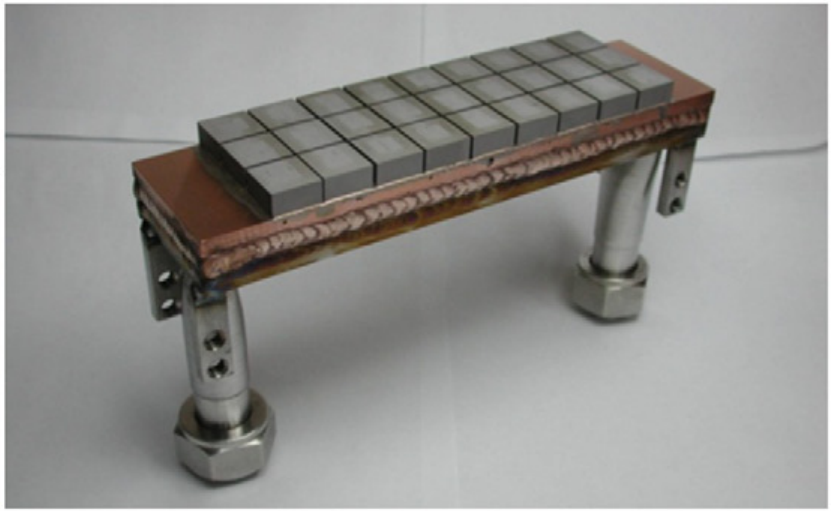
\includegraphics[width=0.7\linewidth]{material/Motojima_tile.png}
    \caption{Фотография плитки, изготовленной для использования в
    ITER~\cite{motojima2015iter}. Медная подложка содержит теплоотводные трубки с
водой.}
	\label{pic::Motojime_tile}
\end{figure}

В экспериментах на токамаке JET прохождение ПЛМ наблюдалось с частотой порядка
$f_{ELM} = 30$ Гц~\cite{coenen2015elm}. 
В ходе прохождения филаментов по поверхности плитки температура поверхности
достигает величин порядка температуры плавления$\left(T_W^{\text{melt}}\right.$ 
$\left.= 3695\text{ К }\right)$~\cite{coenen2015elm}. 
Плавление материала поверхности стенки в современных спецификациях принято как
явление не препятствующее корректной работе реактора, в то время как плавление
всего моноблока, очевидно, является недопустимым явлением\hl{поправить
цитирование: взять конкретное выступление Loarte}~\cite{soukhanovskii23rd}
Так, в работе~\cite{gunn2017surface} сделан вывод о возможности оплавления
поверхности моноблоков дивертора в ходе прохождения ПЛМ во время тестовых сценариев с
использованием $He-D$ смеси\hl{(15 МА)}. При сценариях с использованием $D-T$ смеси
плавление основной части моноблока является неизбежным явлением при прохождении
ПЛМ.

Из последствий плавления поверхностей вольфрамовых плиток можно упомянуть
возможное попадание ионов вольфрама в основной объём плазмы, что даже при малых
концентрациях (порядка $1.0\cdot10^{-5}$ от общего числа атомов\hl{где-то у
Pitts}) делает термоядерный синтез невозможным. Так же, возникают капельные
фракции --- порядка 80 мкм~\cite{coenen2015elm}.

В отсутствие ПЛМ, стационарная температура поверхности дивертора в ITER
ожидается равной $1100-2000$ К в различных областях при нагрузке $q_{tg} = 10$
МВт/м$^2$~\autoref{pic::Motojime_tile}
\begin{figure}[H]
	\centering
	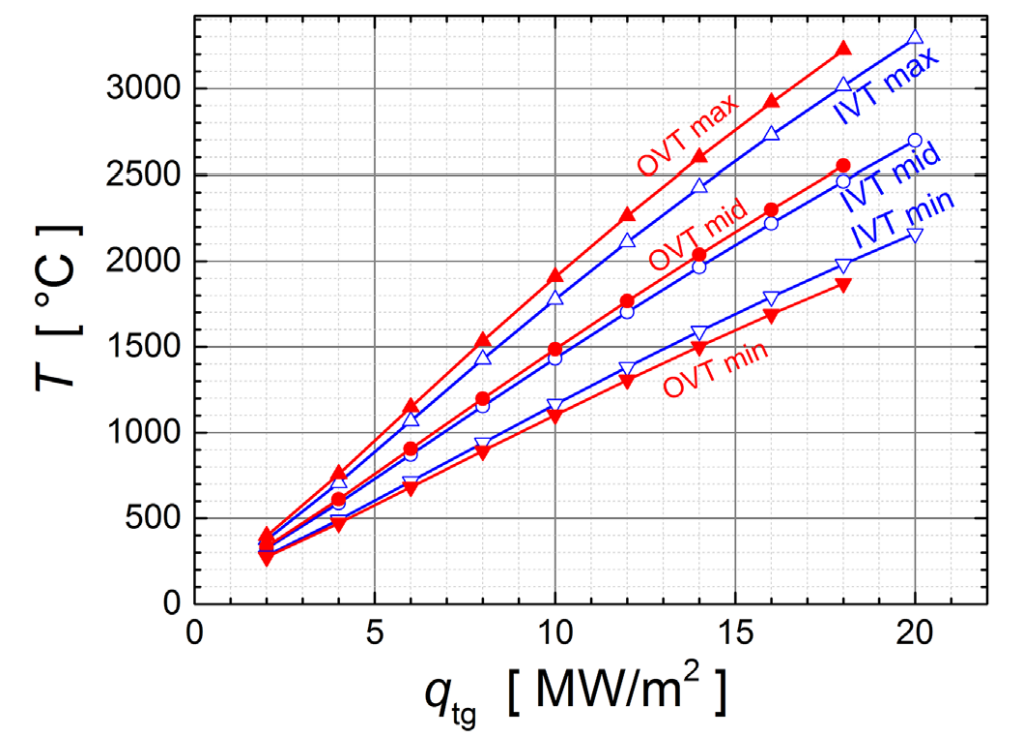
\includegraphics[width=0.7\linewidth]{material/Gunn_temperatures_qtg.png}
    \caption{Результаты моделирования температуры поверхности моноблока
    дивертора в ITER.~\cite{gunn2017surface} OVT --- внешняя вертикальная цель,
IVT --- внутренняя вертикальная цель.}
	\label{pic::Motojime_tile}
\end{figure}

Для задачи поиска значений параметров дебаевского слоя в
термоядерных установках важными являются параметры ПЛМ. ПЛМ могут иметь разные
причины возникновения и имеют соответствующую классификацию. Несмотря на это, 
их принципиальные свойства являются едиными~\cite{spolaore2017electromagnetic}.
Филаменты, являющиеся выбросом плазмы из основного объёма, имеют хорошую
проводимость\hl{порядка проводимости стали}. В соответствии с хорошо описанным
являнием вмораживания магнитных силовых линий в плазму, они являются
''проводниками'' осцилляций электромагнитного поля. На токамаке COMPASS в ходе
экспериментов наблюдались осцилляции магнитного поля~\hl{в какой точке на
стенке?} при прохождении филамента по поверхности плитки.

В работе \cite{spolaore2017electromagnetic} приводятся следующие параметры
осцилляций в ПЛМ: средняя длительность прохода ПЛМ $t_{ELM} = 0.35$ мс, осцилляции магнитного поля
имеют малую амплитуду: $\delta B \approx 0.2$ мТ $\ll~B = 1.15$ Т, но
возникающий из---за них ток через дебаевский слой
значителен~\hl{цитирование laggner с графиком для asdex upgrade?}. Частота сигнала,
распространяющегося внутри филамента имеет характерные частоты порядка
$100$---$240$ КГц~\cite{spolaore2017electromagnetic},~\cite{laggner2016high}, соответствующей характерному
значению альфвеновской частоты $\nu_A$. Отсюда, можно сделать вывод о
необходимости учёта тока смещения в дебаевском слое: найдём частоту, при которой
ток смещения становится порядка тока
проводимости~\eqref{eq::displace_current::1}.
\begin{gather}
    \cfrac{\partial \vec{B}}{\partial t} = \cfrac{4\pi}{c}\vec{j} +
    \cfrac{1}{c}\cfrac{\partial \vec{E}}{\partial t}\\
    \cfrac{1}{c}\cfrac{\partial \vec{E}}{\partial t} \sim \cfrac{\omega}{c}E
    \sim \cfrac{\omega}{c}\cfrac{j}{\sigma}
    \label{eq::displace_current::1}
\end{gather}
\begin{equation}
    \cfrac{\cfrac{\omega}{c}\cfrac{j}{\sigma}}
    {\cfrac{4\pi}{c}j}
    \sim \cfrac{\omega}{4\pi\sigma} 
    \sim \cfrac{\omega}{4\pi\cfrac{ne^2}{m_e}\cfrac{1}{\nu_e}}
    = \cfrac{\omega \nu_e}{\omega_{pe}^2} \sim 1
    \label{eq::displace_current::2}
\end{equation}
При параметрах $n_e = 10^{13}$ см$^{-3}$, $T_e = 100$ эВ, следует, что $\omega
\sim 10^{16}$ с${-1}$. Таким образом, влияние тока смещения является малозначительным,
по сравнению с током проводимости в рассматриваемых сценариях.

При температурах, достигающих температуры плавления, роль термоэлектронной
эмиссии и ее влиянии на регуляцию потоков через дебаевский слой становится
крайне значимым~\cite{takamura1998heat}. Термоэлектронная и вторичная
электронная эмиссии являются основными в экранировании потоков через слой,
ограничивая резкое уменьшение плавающего потенциала поверхности плитки при росте
температуры поверхности. Эмитированные электроны образуют виртуальный катод ---
минимум потенциала в дебаевском слое, способный ''запирать'' частицы возле
поверхности стенки и отражать недостаточно быстрые электроны, идущие со стороны
плазмы. Данное явление известно давно и было аналитически описано в классической
работе~\cite{langmuir1913effect}. 

При возникновении виртуального катода слой кардинально меняет характер изменения
величин с увеличением температуры~\autoref{pic::Moritz_qTs}, прерывая почти экспоненциальный рост тепловой
нагрузки на плитку резким выходом зависимости на ''плато'', значительно
отличающегося от широко принятой оценки теплового
потока~\eqref{eq::qClassicEstimate}~\cite{stangeby2000plasma}.


\begin{equation} 
    q_{plasma} = 8n_{se}c_sT_e 
    \label{eq::qClassicEstimate}
\end{equation}

Так, в работе~\cite{moritz2024simulated} было теоретически и в результате
решения системы уравнений для поиска стационарных параметров дебаевского слоя
показано существование гистерезиса зависимости стационарной температуры
поверхности от начального значения~\autoref{pic::Moritz_hysteresis}. Помимо этого, в этой же работе было показано
существование положительной обратной связи: с ростом температуры тепловая
нагрузка на стенку возрастает ввиду уменьшения $\mid V_f \mid$, что приводит к
тому, что плитку достигает больше электронов из ''медленной'' части
распределения по скоростям. 


\begin{figure}[H]
	\centering
	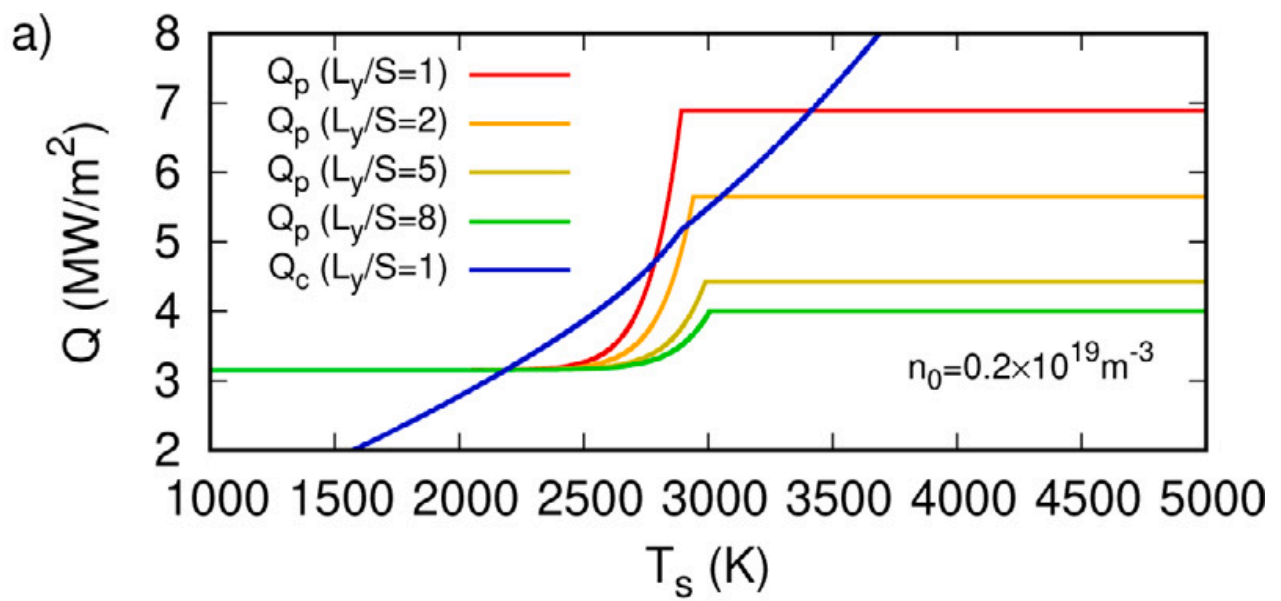
\includegraphics[width=0.7\linewidth]{material/Moritz_qTs.png}
    \caption[]{График зависимости плотности теплового потока на плитку от
    температуры поверхности плитки.~\cite{moritz2024simulated} Параметр $L_y/S$ --- отношение
площади пятна к площади всей поверхности плитки. $Q_p$ --- тепловой поток из
плазмы, $Q_c$ --- мощность теплоотвода, $n_0$ --- плотность плазмы}
	\label{pic::Moritz_qTs}
\end{figure}

\begin{figure}[H]
	\centering
	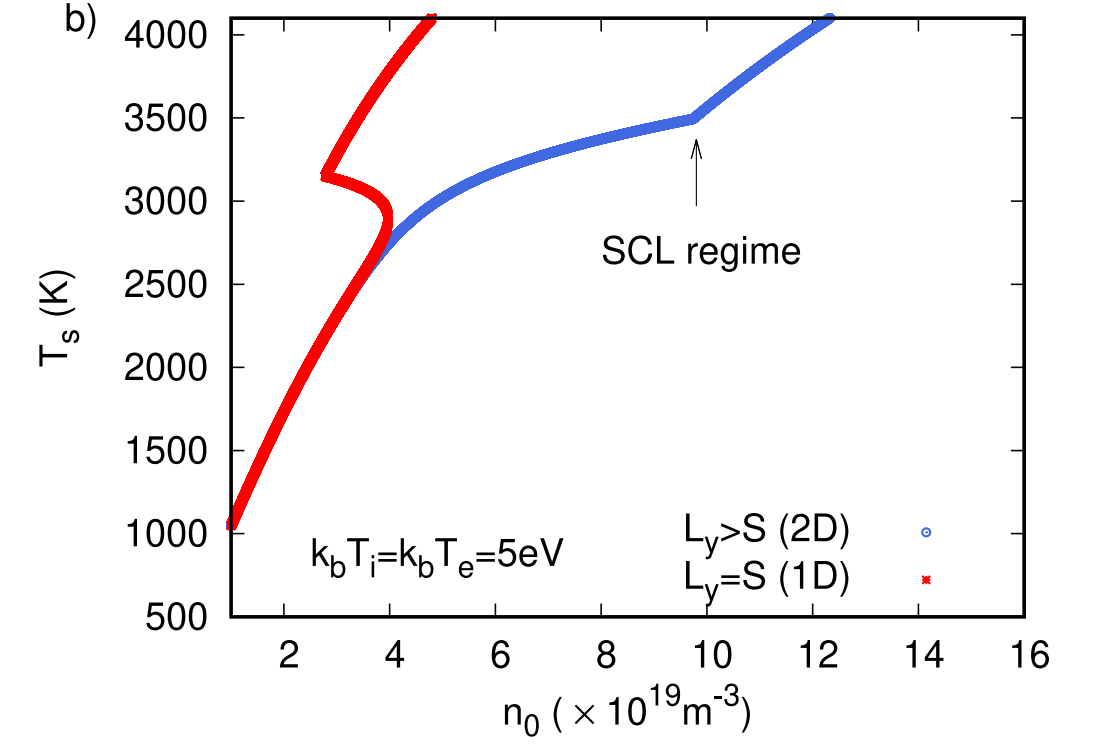
\includegraphics[width=0.7\linewidth]{material/Moritz_hysteresis.png}
    \caption[]{Пример кривой(красная кривая) гистерезиса зависимости
    стационарной температуры~\cite{moritz2024simulated}}
	\label{pic::Moritz_hysteresis}
\end{figure}

В результате PIC симуляций показано наличие осцилляций температуры поверхности
плитки и параметров систему ввиду инерции теплопроводности в материале. Так же 
показано существование ''запертых'' виртуальным катодом частиц.

Отметим\hl{допустимо ли множественное?}, что оценка~\eqref{eq::qClassicEstimate}
справедлива для локального термодинамического равновесия плазмы$\left(T_i =
T_e\right)$ и не учитывает наличия осцилляций электрического поля в дебаевском
слое, наблюдаемого в реальных экспериментах~\cite{kirk2006evolution}. Ввиду
нелинейного характера поведения дебаевского слоя, импеданс в среднем по периоду
осцилляций не равен нулю~\cite{myra2015radio}, что приводит к осцилляциям тока в
слое, и как следствие, тепловых потоков. В совокупности с наличием положительной
обратной связи в системе и инерцией теплопроводимости, это потенциально может
привести к значительному росту усреднённой по периоду осцилляций тепловой
нагрузки на стенку.
%

В современных работах изучено влияние множества факторов и составлены
соответствующие модели, учитывающие конечность
температуры ионов \cite{schwager1993effects}, ~\cite{ou2017heat}, отношения
температуры эмитированных электронов~\cite{sheehan2014effects}, наличие
фотоэлектронной эмиссии, отрицательных ионов~\cite{taccogna2014non}, различных
профилей распределения скоростей частиц~\cite{stangeby1984plasma},
пондеромоторных сил~\cite{takamura1998heat}, столкновительность
слоя~\cite{godyak2002smooth}\hl{и другие}.

Дебаевский слой является структурой с достаточно произвольной границей. Как
правило, принимается, что в данной точке поле равным нулю и справедлив критерий
Бома~\eqref{eq::Bohm_overview}.
\begin{equation}
    \upsilon_i^{se} \ge \sqrt{\cfrac{T_e + \gamma T_i}{m_e}}
    \label{eq::Bohm_overview}
\end{equation}

Однако предположение о равенстве поля на входе в слой является достаточно грубым
--- плазма начинает экранирует поле существующее в дебаевском слое на конечном
расстоянии. Так, в работе~\cite{godyak2002smooth} введено более общее
определение, основанное на данном замечании. В данной работе применяется
''классическое'' предположение о равенстве поля нулю на входе в слой.

Другая важная характеристика дебаевского слоя --- толщина, как правило
оценивается согласно классической формуле
Чайлда---Ленгмюра~\eqref{eq::Child_Langmuir_width}
\begin{equation}
    \lambda = \cfrac{1}{3\pi}\left(enV\right)^{-1/2}\left(\cfrac{2e}{m_e}\right)^{1/4}
    \label{eq::Child_Langmuir_width}
\end{equation}

Данная оценка так же сделана в достаточно грубых приближениях: в слое
отсутствуют электроны и начальная скорость ионов равна нулю. В
работе~\cite{chabert2014size} получена более точная оценка, учитывающая данные
факторы.\hl{графики}

Классический режим работы слоя известен давно и часто подразумевается при
использовании классических оценок теплового потока~\eqref{eq::qClassicEstimate}
и значения плавающего потенциала.~\hl{добавить работы}.

В работе~\cite{campanell2018alternative} рассматривается альтернативный
инвертированный режим работы слоя. В данной режиме слой монотонен, но
электростатический потенциал в дебаевском слое всюду больше потенциала плазмы.
Данный режим нестабилен относительно возмущений плотности, но имеет конечное
время релаксации к прежнему состоянию. В других работах автор
~\cite{campanell2016strongly},~\cite{campanell2020possible} отмечает, что
вообще говоря, режим объёмного экранирования зарядом не является устойчивым и
ввиду накопления ионов в промежутке между виртуальным катодом и поверхностью,
переходит в инвертированный режим. Данный режим обеспечивает \hl{''детачмент''}:
возле поверхности плитки образуется промежуточная область с холодной
плазмой.~\hl{подробнее о том зачем это}.

\pagebreak

\section{Описание модели}

\qquadВ работе рассматривается полностью ионизированная, идеальная неравновесная 
плазма, состоящая из положительно заряженных однозарядных ионов и электронов. 
В токамаках, где поддерживается низкое давление($\sim 10^{-8}$ торр), плазма является неравновесной и температура
электронов много больше температуры ионов и атомов: $T_a \approx T_i < T_e$, отсюда, в модели принято: $T_i = 0$. Электроны, приходящие из плазмы,
всюду находятся в равновесии и имеют распределение Максвелла. Плазма квазинейтральна вплоть
до входа в дебаевский слой: $n_i^{se} = n_e^{se} = n^{se}$.


\qquadСтенка имеет координату $x = 0$, точки, соответствующие слою и
плазме, имеют положительные координаты~\autoref{pic::model}.
На стенке устанавливается квазистационарное равновесие: сумма токов равна 0 и стенка имеет установившийся плавающий потенциал $V_f$, имеющий
характерное значение порядка $eV_{char} = -3T_e$ и эффективно отражающий поток электронов из плазмы. Знак плавающего
потенциала('нуль' потенциала принят на $x\rightarrow + \infty$) 
и монотонность электростатического потенциала в
слое определяются режимом работы слоя.

\begin{figure}
	\centering
	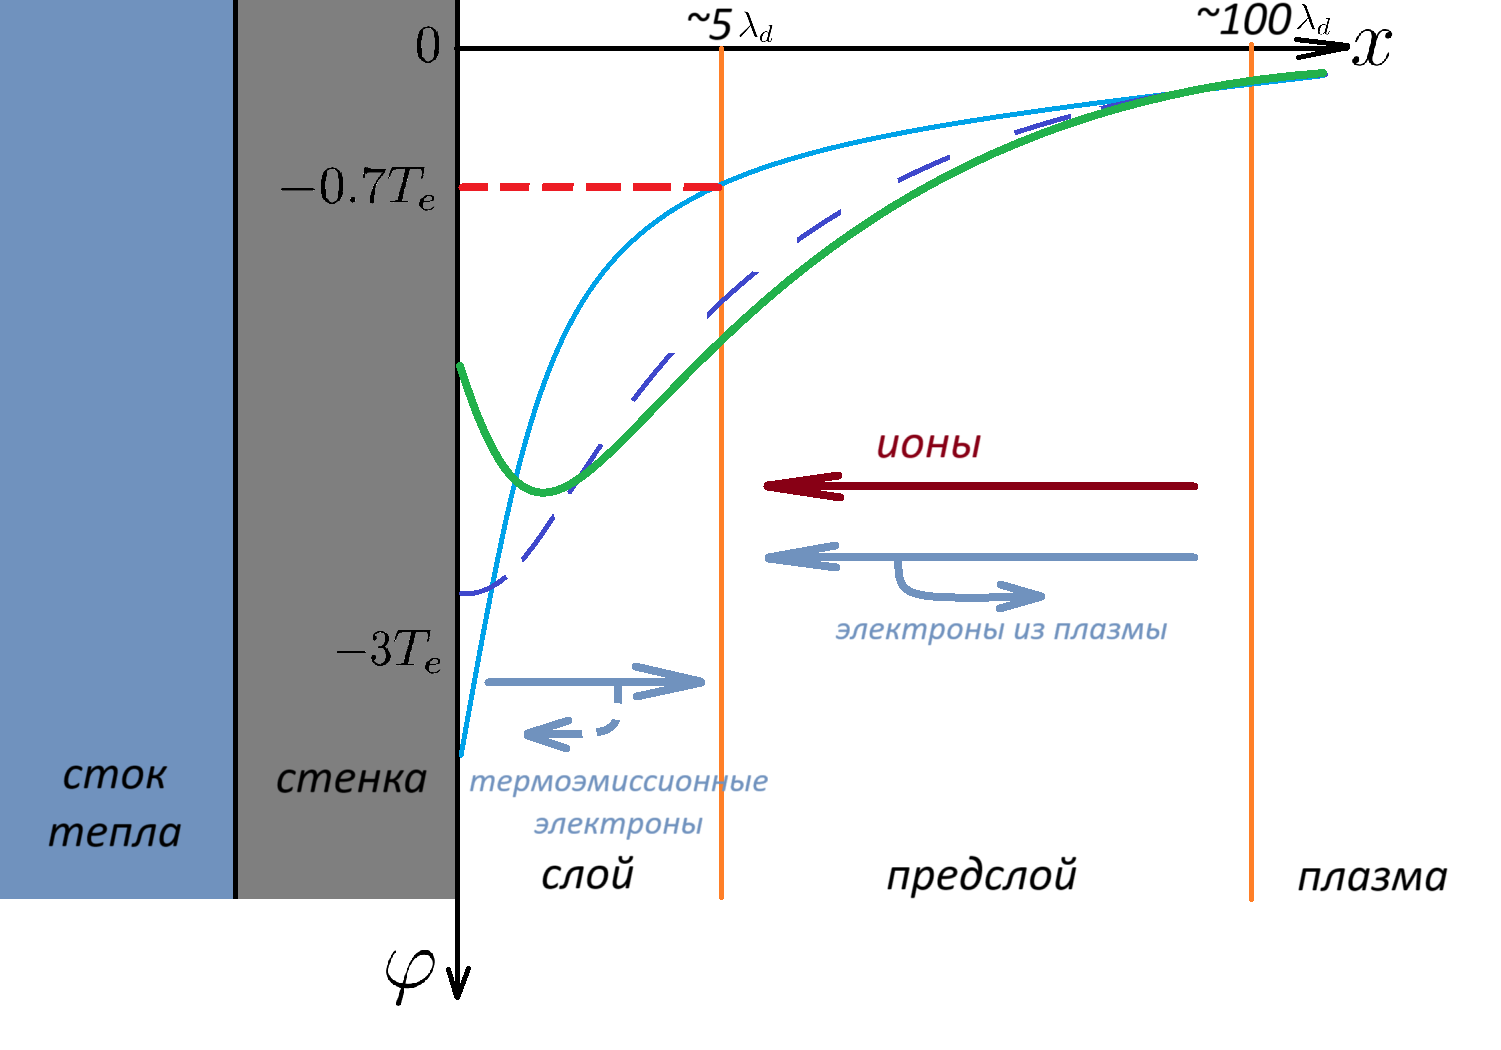
\includegraphics[width=0.7\linewidth]{material/model.png}
	\caption{Модель слоя. Линии соответствуют различным режимам работы: голубая --- классический, фиолетовая прерывистая --- переходный, зеленая --- ограниченный объёмным зарядом. $\lambda_d$ --- радиус Дебая}
	\label{pic::model}
\end{figure}

\qquadТермоэлектронная эмиссия описывается законом Ричардсона---Дешмена. В работе так же рассмотрено влияние эффекта Шоттки~\eqref{eq::Shottky}:
\begin{subequations}
    \begin{align}
        j_{te} &= aT_s^2\exp{\cfrac{-e(\varphi_{out} + \Delta\varphi_{Sh})}{T_s}}
        \\ \Delta\varphi_{Sh} &= -\sgn{E_x}\cdot\sqrt{e\lvert E_x\rvert}
    \end{align}
    \label{eq::Shottky}
\end{subequations}


\qquadОбразовавшаяся структура может быть разделена на \\несколько областей: у стенки находится дебаевский слой, в котором нарушена квазинейтральность плазмы
и присутствует сильное поле. Для образования данной структуры ионы должны иметь достаточно большую скорость, которую они набирают
в предслое --- области между плазмой и слоем. 
Значение потенциала входа в дебаевской слой не равно нулю. Уменьшение потенциала соответствует разгону 
ионов до скорости $\upsilon_0$, требуемой для выполнения критерия Бома~\cite{stangeby2000plasma}
существования неосциллирующего решения уравнения Пуассона в слое:
\begin{equation}
	\varphi_{se} = \cfrac{-m_i\upsilon_0^2}{2e}
	\label{eq::Bohm}
\end{equation}

\qquadРазмеры предслоя гораздо больше размеров слоя(порядка $100$ радиусов Дебая для предслоя, $\sim 5$ --- для слоя)

\qquadВ работе рассмотрены следующие режимы:
\begin{itemize}
    \item Классический --- присутствует поле возле стенки, поле в слое монотонно возрастает
    \item Ограниченный объёмным зарядом --- ввиду активной эмиссии электронов со стенки возникает виртуальный катод в слое, приводящий к экранированию потока термоэмиссионных электронов
\end{itemize}


\subsection{Классический режим}
\qquadСлой является монотонным, ускоряя термоэмиссионные \\электроны. Температура термоэмиссионных электронов 
принята равной температуре поверхности стенки $T_s$:
\begin{equation}
	f(\upsilon, x) = n_{te}^s\sqrt{\cfrac{m_e}{2\pi T_s}}\exp{\left(\cfrac{e(\varphi - (V_f + \varphi_{se}))}{T_s}\right)}\theta(\upsilon - \upsilon_{M, te}(x))
	\label{eq::themionic_distribution}
\end{equation}
где $\upsilon_{M, te(x)}$ --- минимальная скорость эмитированных термоэлектронов:
\begin{equation}
	\upsilon_{M, te(x)} = \sqrt{\cfrac{2e(\varphi - (V_f + \varphi_{se}))}{m_e}}
	\label{eq::min_thermionic_electrons_velocities}
\end{equation}

Составим систему относительно неизвестных $n_e^{se}, \left(\cfrac{\partial \varphi}{\partial x}\right)_s, V_f, \varphi_{se}$. Переменные $n_i^{se}, T_s$ 
приняты постоянными и заранее заданными.

\qquadМодули токов на поверхности плитки: 
\begin{subequations}
	\begin{align}
		j_i^s &= en_i^{se}\upsilon_0\\
        j_e^s &= \cfrac{1}{4}en_e^{se}\upsilon_{e}^{th}\exp{\left(\cfrac{eV_f}{T_e}\right)}\\
		j_{te}^s &= aT_s^2\exp{\left(\cfrac{-e(\varphi_{out} + \Delta\varphi_{Sh})}{T_s}\right)}
	\end{align}
	\label{eq::j_sum_classic}
\end{subequations}

\qquadТоки на поверхность плитки квазистационарно уравновешены:
\begin{equation}
	0 = j_i^s - j_e^s + j_{te}^s
	\label{eq::quasineutral_j_balance}
\end{equation}

\begin{equation}
    V_f = \cfrac{T_e}{e}\ln{\left\{
        \sqrt{\cfrac{2\pi m_e}{m_i}}\cfrac{n_i^{se}}{n_e^{se}} 
    + \cfrac{j_s}{\cfrac{1}{4}en_e^{se}\upsilon_e^{th}}
\right\}}
	\label{eq::quasineutral_j_balance}
\end{equation}

При $T_s \rightarrow 0$~\eqref{eq::quasineutral_j_balance} переходит в классическое выражение~\eqref{eq::canonical::quasineutral_j_balance}~\cite{chen1984introduction}:
\begin{equation}
    V_f = \cfrac{T_e}{2e}\ln{\left\{
    \cfrac{2\pi m_e}{m_i}
\right\}}
	\label{eq::canonical::quasineutral_j_balance}
\end{equation}

Вторым уравнением системы является критерий Бома для составленной модели. 
Примем, что вход в слой соответствует точке, где скорость ионов достигает
минимально разрешенной критерием Бома скорости, т.е. в этой точке среда квазинейтральна:

\begin{equation}
	n_i^{se} = n_e^{se} + n_{te}^s\erfc\left(\sqrt{\cfrac{-eV_f}{T_s}}\right)\exp{\left[\cfrac{-eV_f}{T_s}\right]}
	\label{eq::quasineutrality_classic}
\end{equation}

\qquadТ.к. термоэлектроны подчиняются максвелловскому распределению, 
плотность электронов термоэлектронной эмиссии на поверхности плитки определена как:

\begin{equation}
    n_{te}^s = \cfrac{j_{te}^s}{\cfrac{1}{4}e\upsilon_{te}^{th}}
	\label{eq::nte_s_classic}
\end{equation}

Ионы, имеющие одинаковую скорость, можно описать при помощи закона сохранения энергии:

\begin{equation}
	\upsilon_i(x) = \upsilon_0\sqrt{1 - \cfrac{2e(\varphi-\varphi_{se})}{m_i\upsilon_0^2}}
\end{equation}
Тогда, из уравнения непрерывности в отсутствиe процесса накопления заряда в слое:

\begin{equation}
	\cfrac{dj_i}{dx} = 0
\end{equation}
cледует:

\begin{equation}
	n_i(x) = n_i^{se}\cfrac{1}{\sqrt{1 - \cfrac{2e(\varphi-\varphi_{se})}{m_i\upsilon_0^2}}}
\end{equation}

Критерий Бома может быть получен из разложения в ряд Тейлора правой части уравнения Пуассона~\eqref{eq::Poisson_classic} по 
малому параметру $\Delta = \varphi - \varphi_{se} \ll T_s \ll T_e$.

\begin{equation}
	\begin{split}
	\cfrac{d^2\varphi}{dx^2} = -4\pi e\left(n_i^{se}\cfrac{1}{\sqrt{1 - \cfrac{2e(\varphi-\varphi_{se})}{m_i\upsilon_0^2}}} - n_e^{se}\exp{\cfrac{e(\varphi - \varphi_{se})}{T_e}} -\right.
	\\ \left.- n_{te}^w\erfc\left[\sqrt{\cfrac{e(\varphi - (\varphi_{se} + V_f))}{T_w}}\right]\exp{\cfrac{e(\varphi - (\varphi_{se} + V_f))}{T_w}}\right)
	\end{split}
	\label{eq::Poisson_classic}
\end{equation}

\begin{equation}
	\begin{split}
	&\cfrac{d^2\varphi}{dx^2} = -4\pi\left(n_i^{se}\cfrac{1}{m_i\upsilon_0^2} - n_e^{se}\cfrac{1}{T_e} - \right. 
		\\ &\left. - n_{te}^w\cfrac{1}{T_w}\left[\exp{\cfrac{-eV_f}{T_w}}\erfc{\sqrt{\cfrac{-eV_f}{T_w}}} - \sqrt{\cfrac{1}{\pi}}\cfrac{1}{\sqrt{\cfrac{-eV_f}{T_w}}}\right]\right)\Delta \ge 0
	\end{split}
    \label{eq::Poisson_Bohm_classic}
\end{equation}

Правая часть уравнения~\eqref{eq::Poisson_Bohm_classic} должна быть больше 0 для существования неосциллирующего решения, следовательно,
выражение в скобках должно быть меньше 0, откуда получаем выражение для критерия Бома:

\begin{equation}
	m_i\upsilon_0^2 \ge \cfrac{n_i^{se}T_eT_w}{n_e^{se}T_w + n_{te}^wT_e\left[\erfc{\sqrt{\cfrac{-eV_f}{T_w}}}\exp{\cfrac{-eV_f}{T_w}} - \sqrt{\cfrac{1}{\pi}}\cfrac{1}{\sqrt{\cfrac{-eV_f}{T_w}}}\right]}
	\label{eq::Bohm_classic}
\end{equation}

Полученное выражение~\eqref{eq::Bohm_classic} при $T_s\rightarrow0$ переходит в классическое\cite{stangeby2000plasma}:
\begin{equation}
    \upsilon_0 \ge \sqrt{\cfrac{T_e}{m_i}}
	\label{eq::canonical::Bohm_classic}
\end{equation}

\qquadЗамыкающим систему является проинтегрированное между входом в слой и поверхностью стенки уравнение Пуассона:

\begin{equation}
	\begin{split}
        \left(\cfrac{d\varphi}{dx}\right)^2_s &= 8\pi\left(n_i^{se}m_i\upsilon_0^2\sqrt{1 - \cfrac{2e(\varphi-\varphi_{se})}{m_i\upsilon_0^2}}\right. + 
	   \\ &+ n_e^{se}T_e\exp{\cfrac{e(\varphi-\varphi_{se})}{T_e}} + n_{te}^sT_s \times
	\\ & \times \left[\exp{\cfrac{e(\varphi - (V_f + \varphi_{se}))}{T_s}}\erfc{\sqrt{\cfrac{e(\varphi - (V_f + \varphi_{se}))}{T_s}}} \right.+
	\\ &\left. + \cfrac{2}{\sqrt{\pi}}\sqrt{\cfrac{e(\varphi - (V_f + \varphi_{se}))}{T_s}}\right]\Bigr|_{\varphi_{se}}^{V_f + \varphi_{se}}\Bigg)
	\end{split}
    \label{eq::Poisson_classic_wall}
\end{equation}

\qquadТаким образом, получена система~\eqref{eq::quasineutrality_classic},~\eqref{eq::quasineutral_j_balance},~\eqref{eq::Poisson_classic_wall},~\eqref{eq::Bohm_classic} относительно четырёх неизвестных: $n_e^{se}$, 
$V_f$, $\varphi'(x = 0), \varphi_{se}$ при $T_s, n_i^{se}$ взятых как параметры ($n_{te}^s$ --- производный параметр)

Для решения нестационарной задачи с учётом теплопроводности в материале стекни требуется выражение для теплового потока.
Тепловой поток состоит из нескольких компонент:

\begin{equation}
    q = q_i + q_e + q_{te}
\end{equation}

В типичных сценариях работы токамака $T_s ~\approx0.3\text{ эВ} \ll T_e \approx 200\text{ эВ}$, что позволяет пренебречь 
тепловым потоком термоэмиссионных электронов:

\begin{equation}
    q_{te} = j_{te}\cdot\cfrac{2T_s}{e} \propto T_s^{3/2} \ll T_e^{3/2} \proptoinverse q_e,q_i
\end{equation}

Таким образом:

\begin{equation}
    q = n_i^{se}\upsilon_0\left(\cfrac{m_i\upsilon_0^2}{2} - eV_f\right) + \cfrac{1}{4}n_e^{se}\upsilon_e^{th}\cdot2T_e\exp\left[\cfrac{eV_f}{T_e}\right]
\end{equation}

\subsection{Режим ограничения объёмным зарядом}

\qquadС увеличением электронной эмиссии со стенки, начиная с некоторого критического значения, 
возникает виртуальный катод --- минимум потенциала, где как следствие, отсутствует поле.
Возникающая структура регулирует ток частиц в обе стороны, в частности, возникает отражение
эмитированных электронов на разности потенциалов $\varphi_{vc} - \varphi_s < 0$ 
обратно на стенку. Таким образом, в системе уравнений возникает дополнительная 
неизвестная --- $\varphi_{vc}$.

\qquadТок прошедших виртуальный катод электронов из плазмы определяется соответствующим током 
на виртуальном катоде, т.к. между стенкой и виртуальным катодом электроны отражаются на 
стенку.

\qquadДля потока электронов в области $x > x^{vc}$ верно уравнение неразрывности:
\begin{equation}
	dj_{te}(\upsilon_s) = e\upsilon_s n_{te}^s \cdot f(\upsilon_s) d\upsilon_s = e\upsilon(x, \upsilon_s)\cdot dn_{te}(x)
\end{equation}

\qquadОтсюда:
\begin{equation}
	n_{te} = n_{te}^s \int\limits_{\upsilon_{vc}}^{\infty}\,d\upsilon_s \cfrac{\upsilon_s f(\upsilon_s)}{\upsilon}
	\label{n_thermionic}
\end{equation}
где $\upsilon_{vc}$ --- минимальная необходимая для преодоления виртуального катода 
при движении со стенки скорость электронов.

% \qquadСтоит отметить, что $n_{te}^s$ в случае экранирования объёмным зарядом(как и в классическом 
% случае) является концентрацией электронов в потоке, эмитируемом со стенки.

\qquadТ.к. слой считается бесстолкновительным, из закона сохранения энергии выразим скорость  
электронов в точке --- $\upsilon$:
\begin{equation*}
	\cfrac{m_e(\upsilon_s)^2}{2} - e(V_f + \varphi_{se}) = \cfrac{m_e\upsilon^2}{2} - e\varphi
\end{equation*}

\begin{equation}
	\upsilon = \upsilon_s\sqrt{1 + \cfrac{2e(\varphi - (V_f + \varphi_{se}))}{m_e(\upsilon_s)^2}}
	\label{upsilon_th}
\end{equation}

\qquadИнтегрируя, получим:
\begin{equation}
	n_{te}(\varphi) = n_{te}^s\erfc{\sqrt{\cfrac{e(\varphi - \varphi_{vc})}{T_s}}}\exp{\cfrac{e(\varphi - (V_f + \varphi_{se}))}{T_s}}
\end{equation}

В области между поверхностью плитки и виртуальным катодом, примем, что ансамбль термоэлектронов находится в равновесии и 
распределение является максвелловским.

Составим систему уравнений аналогичную полученной в классическом режиме: неизвестными приняты $n_e^{se}, \varphi_{se}, \left(\cfrac{\partial \varphi}{\partial x}\right)_s, V_f, V_{vc}$,
заданными константами --- $n_i^{se}, T_s$.

Область между виртуальным катодом и входом в дебаевский слой можно рассматривать 
как при классическом режиме: основное отличие заключается в том, что выражение для 
термоэмиссионного тока теперь содержит множитель ''отсечки''. Таким образом, заменив 
в выражениях $V_f$ на $V_{vc}$ и учтя отражение термоэмиссионных электронов, получим 
аналог прежних четырёх уравнений системы.

Замыкающее уравнение может быть получено интегрированием уравнения Пуассона в области 
между поверхностью плитки и виртуальным катодом:
\begin{equation}
    \begin{split}
        \left(\cfrac{d\varphi}{dx}\right)^2_s &= 8\pi\left[n_im_i\upsilon_0^2\sqrt{1 - \cfrac{2e(\varphi - \varphi_{se})}{m_i\upsilon_0^2}} + \right.
        \\ &+ n_e^{se}T_e\exp{\cfrac{-e\varphi_{se}}{T_e}}\left(\exp{\cfrac{e\varphi}{T_e}}\erfc{\sqrt{\cfrac{e(\varphi - (V_{vc} + \varphi_{se}))}{T_e}}} \right.+ 
        \\ &+ \left. \cfrac{2}{\sqrt{\pi}}\exp{\cfrac{e(V_{vc} + \varphi_{se})}{T_e}}\sqrt{\cfrac{e(\varphi - (V_{vc} + \varphi_{se}))}{T_e}}\right) + 
        \\ &+ \left. n_{te}^sT_s\exp{\cfrac{e(\varphi - (V_f+\varphi_{se}))}{T_s}}\right]\Bigg|_{V_{vc} + \varphi_{se}}^{V_f + \varphi_{se}}
    \end{split}
    \label{eq::Poisson_SCL_alpha}
\end{equation}

Выражение для теплового потока имеет вид:
\begin{equation}
    q = n_i^{se}\upsilon_0\left(\cfrac{m_i\upsilon_0^2}{2} - eV_{vc}\right) + \cfrac{1}{4}n_e^{se}\upsilon_e^{th}\cdot2T_e\exp\left[\cfrac{eV_{vc}}{T_e}\right]
\end{equation}



\subsection{Результаты моделирования}
Результаты решения системы в безразмерных единицах при типичных условиях представлены на~\autoref{pic::Model::results::Te-200eV_ne-1e13cm^-3}. 
Полученные значения согласуются с классическими~\cite{hobbs1967heat} при малых значениях $T_s$: $V_f \approx -2.7$.

Наибольший интерес представляет тот факт, что при переходе в режим экранирования объёмным зарядом, ток термоэлектронной эмиссии 
идеально экранируется виртуальным катодом. Значение потенциала виртуального катода постоянно при изменении температуры, 
плавающий потенциал линейно растёт при увеличении температуры поверхности плитки.

Уменьшение $\varphi_{se}$ с ростом температуры $T_s$ соответствует увеличению потока ионов на плитку. Приращение потока термоэлектронной эмиссии 
приводит к эффективному росту плавающего потенциала $V_f$. Согласно~\eqref{eq::quasineutral_j_balance} и~\eqref{eq::j_sum_classic}:
\begin{equation}
    j_e \propto \exp{\left\{{V_f}\right\}} \propto \sqrt{\cfrac{2\pi m_e}{m_i}}\cfrac{n_i^{se}}{n_e^{se}} + \cfrac{j_s}{\cfrac{1}{4}en_e^{se}\upsilon_e^{th}} 
\end{equation}

\hl{В общем случае, $n_e^{se} \slashed{\propto} j_s$, что приводит к тому, что рост термоэлектронной эмиссии не обязан быть полностью скомпенсированным 
пропорциональным увеличением потока электронов из плазмы. Однако, при фиксированном $\varphi_{se}$ решение системы с исключенным для устранения 
переопределенности критерием Бома возможно, что и будет применено далее.}

По полученному решению построен график зависимости $q(T_s)$~\autoref{pic::Model::results::q_Te-200eV_ne-1e13cm^-3}. При малых температурах тепловой поток 
согласуется с классическим результатом~\cite{stangeby2000plasma}

Распределение потенциала в дебаевском слое может быть получено решением уравнения Пуассона в слое. 
На~\autoref{pic::Model::results::Poisson_Te-200eV_ne-1e13cm^-3} приведено решение для режима объёмного экранирования. Разность потенциалов 
между поверхностью стенки и виртуальным катодом является величиной порядка $T_s - T_{trans}$.

\begin{figure}[H]
	\centering
	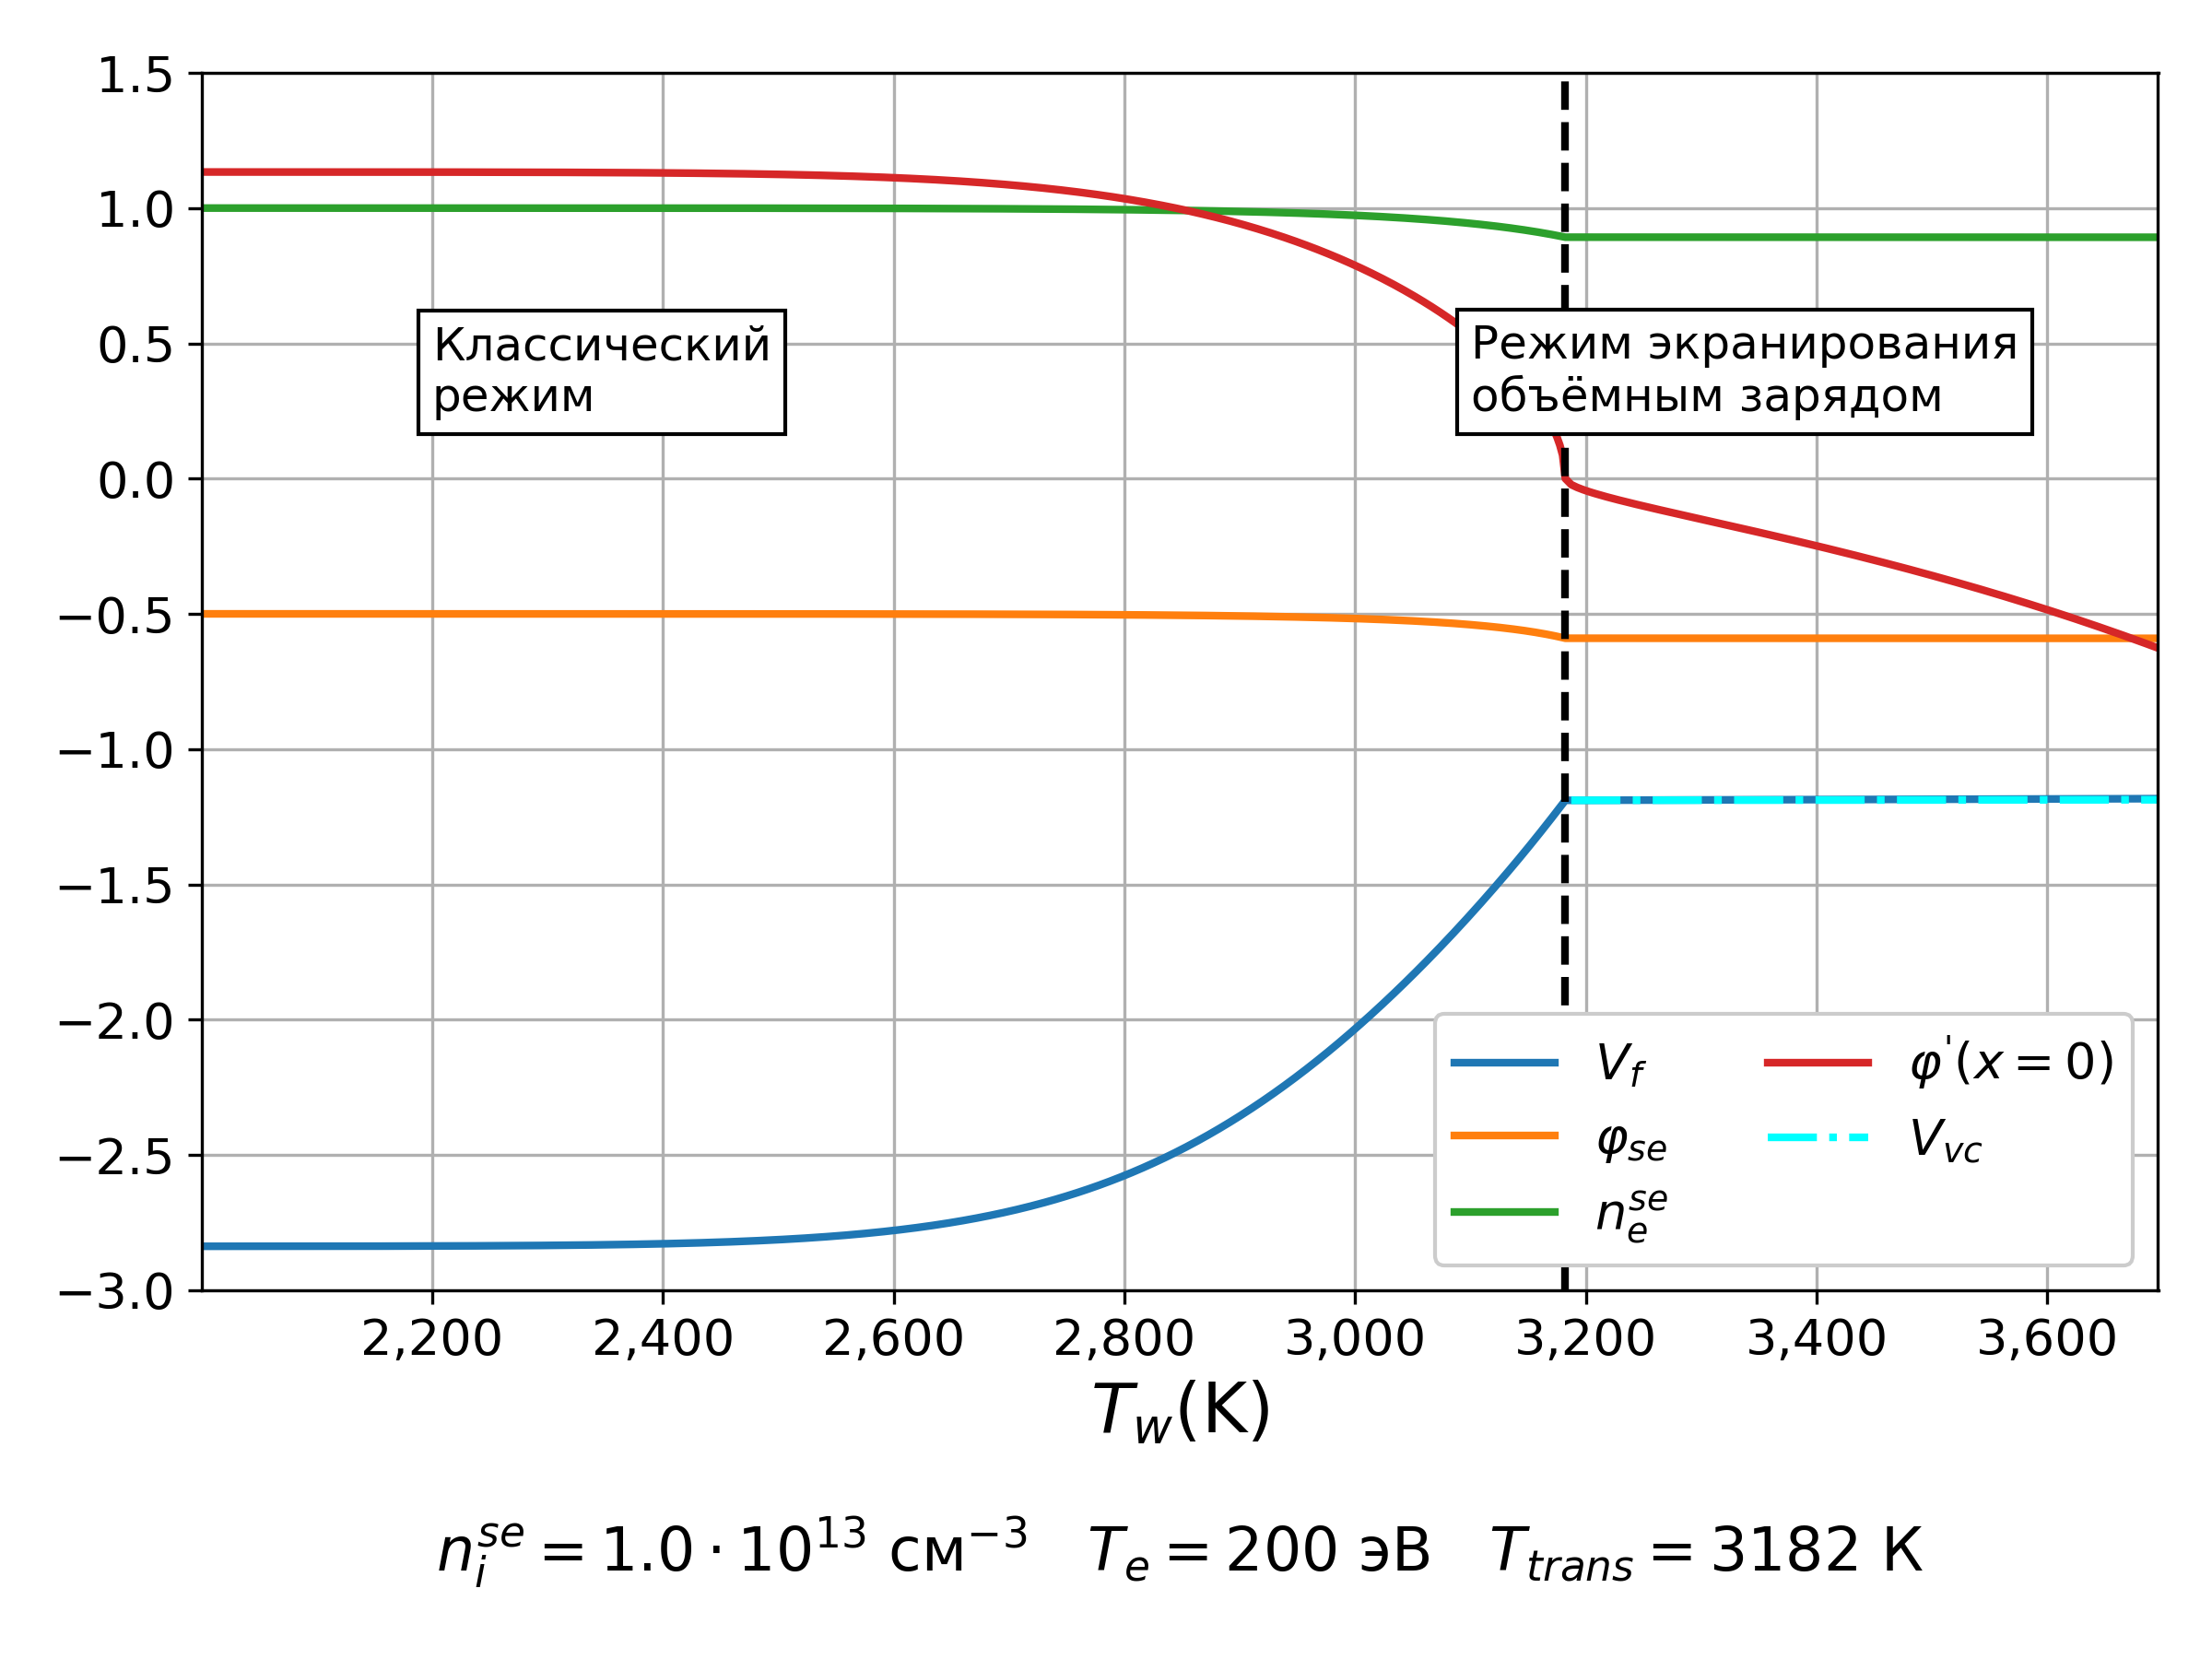
\includegraphics[width=0.7\linewidth]{material/Te=200eV_nse=1.0e13.png}
    \caption[]{График решения систем для поиска параметров дебаевского слоя при заданных $n_i^{se}, T_s$}
	\label{pic::Model::results::Te-200eV_ne-1e13cm^-3}
\end{figure}

\begin{figure}[H]
	\centering
	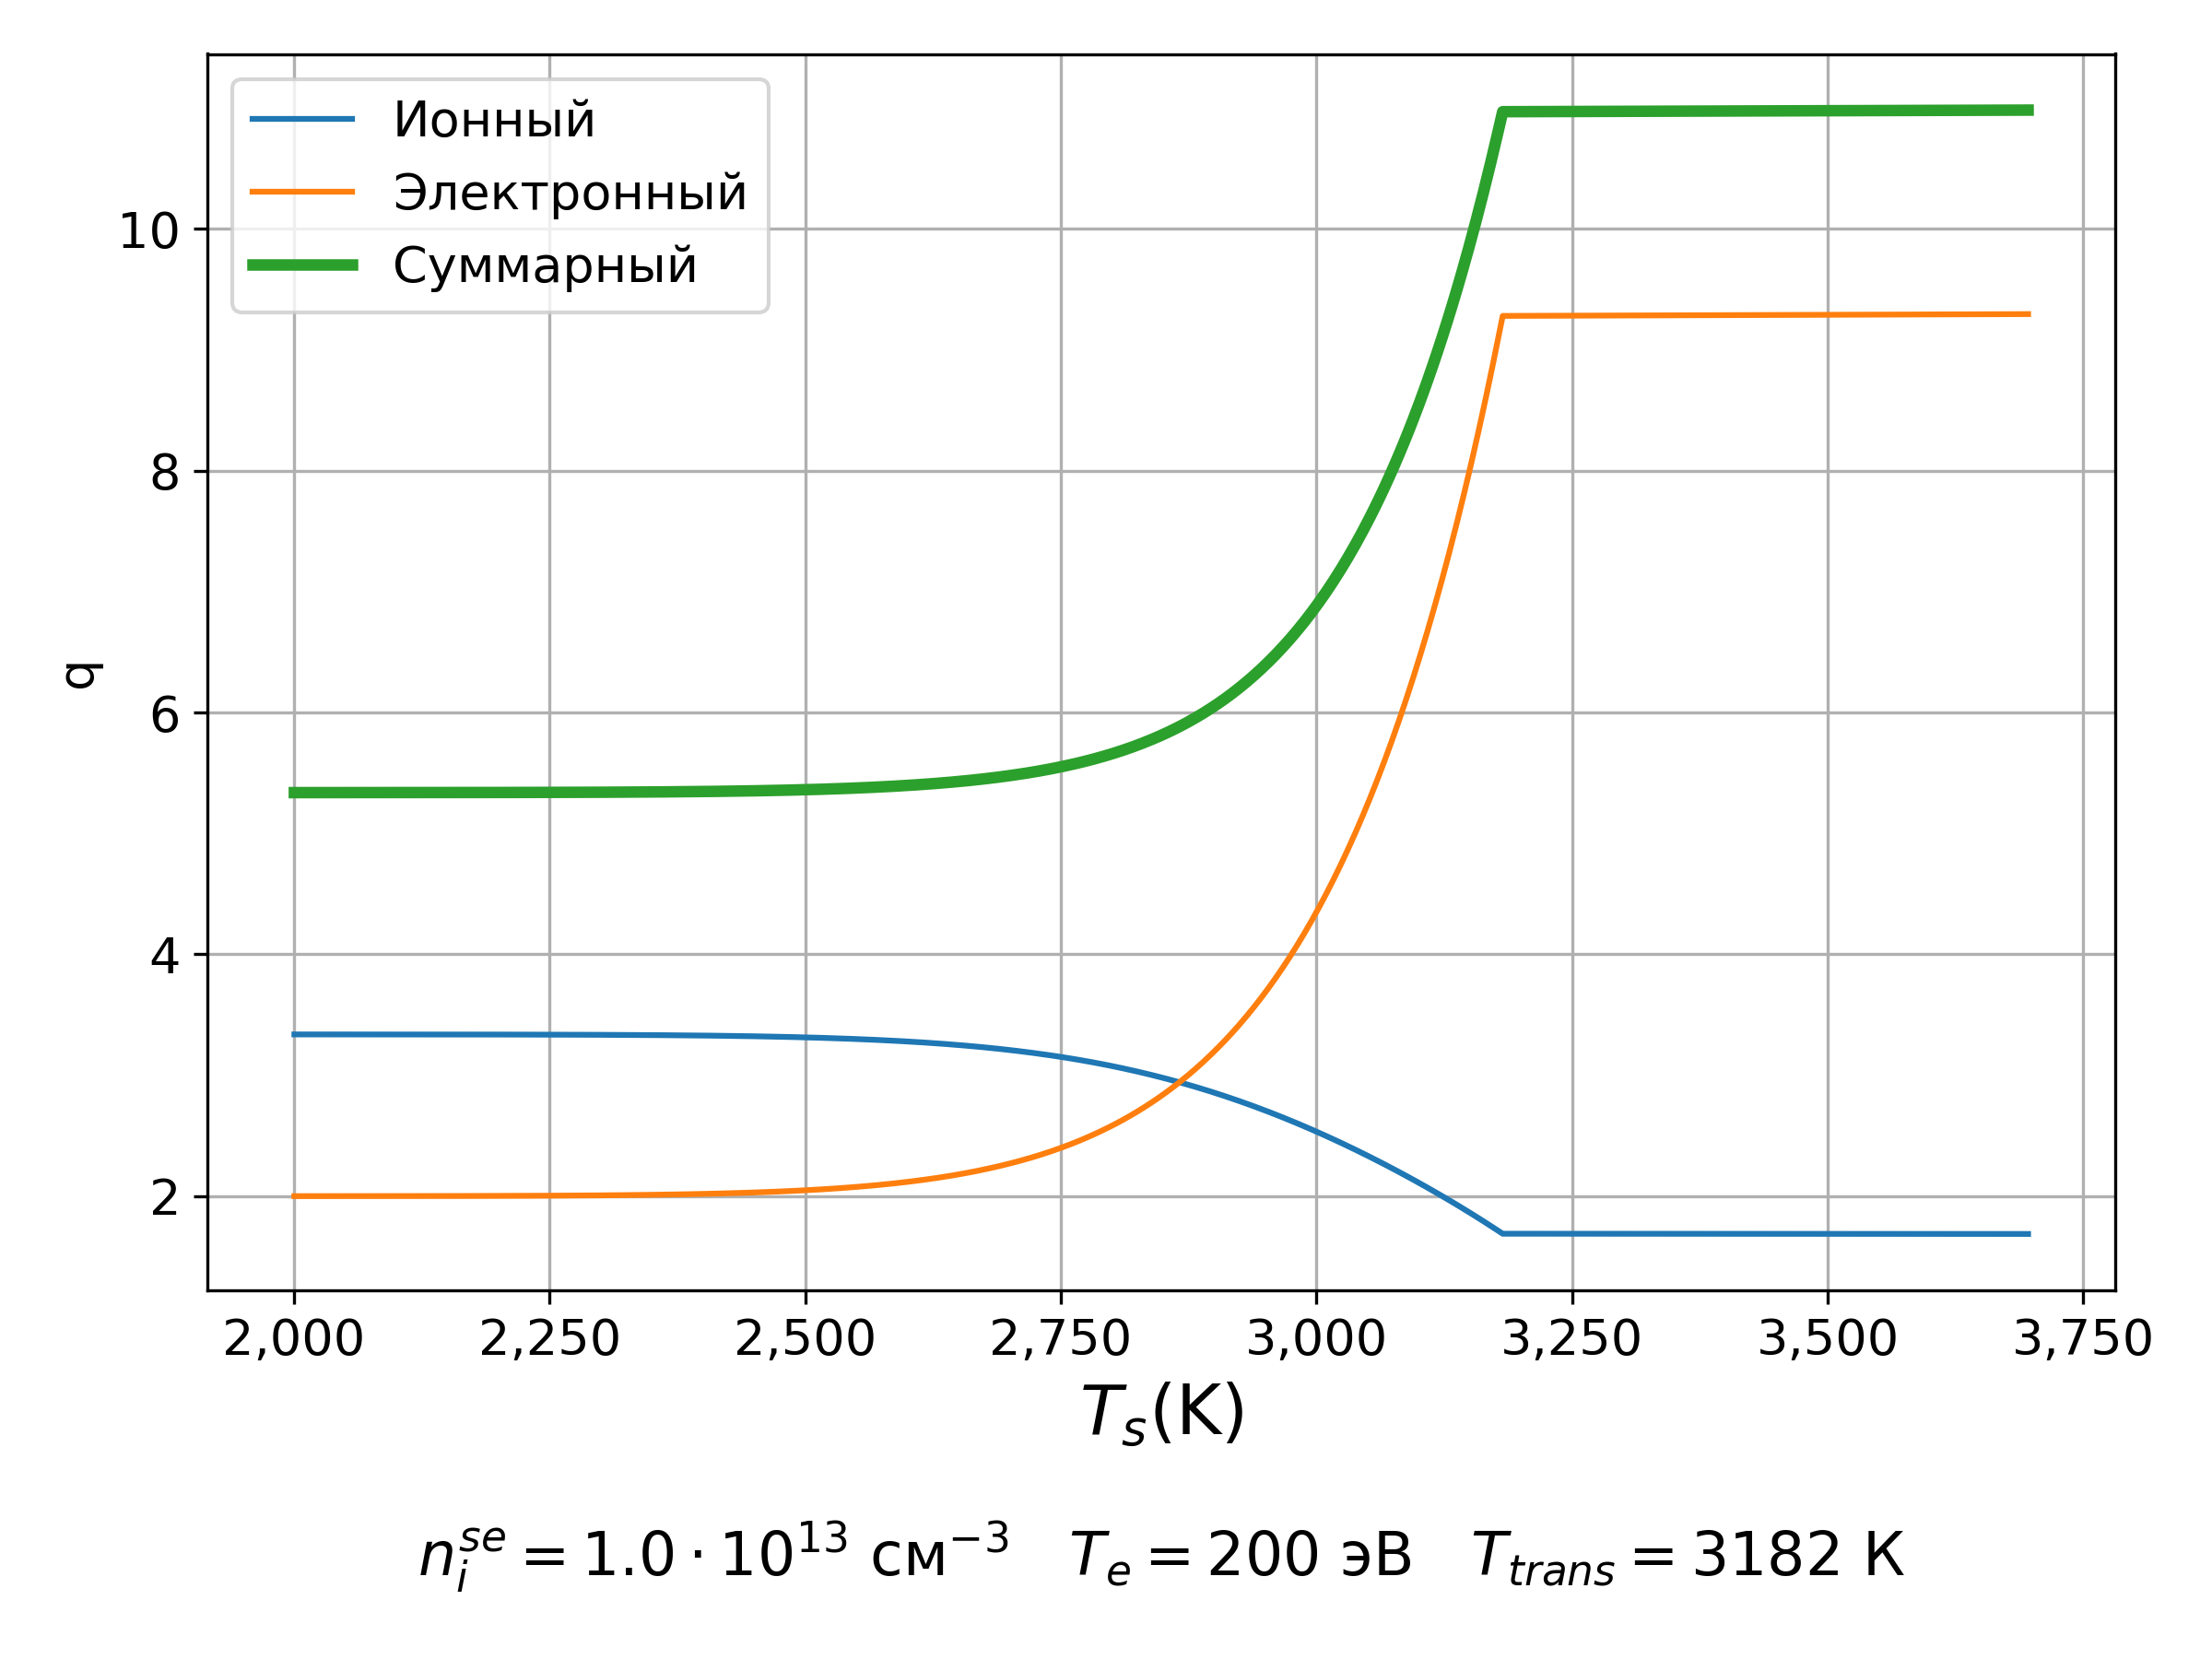
\includegraphics[width=0.7\linewidth]{material/q_plot_Te=200eV_nse=1.0e13.png}
    \caption[]{График зависимости теплового потока от температуры поверхности плитки}
	\label{pic::Model::results::q_Te-200eV_ne-1e13cm^-3}
\end{figure}

\begin{figure}[H]
	\centering
	\begin{subfigure}{\textwidth}
		\centering
	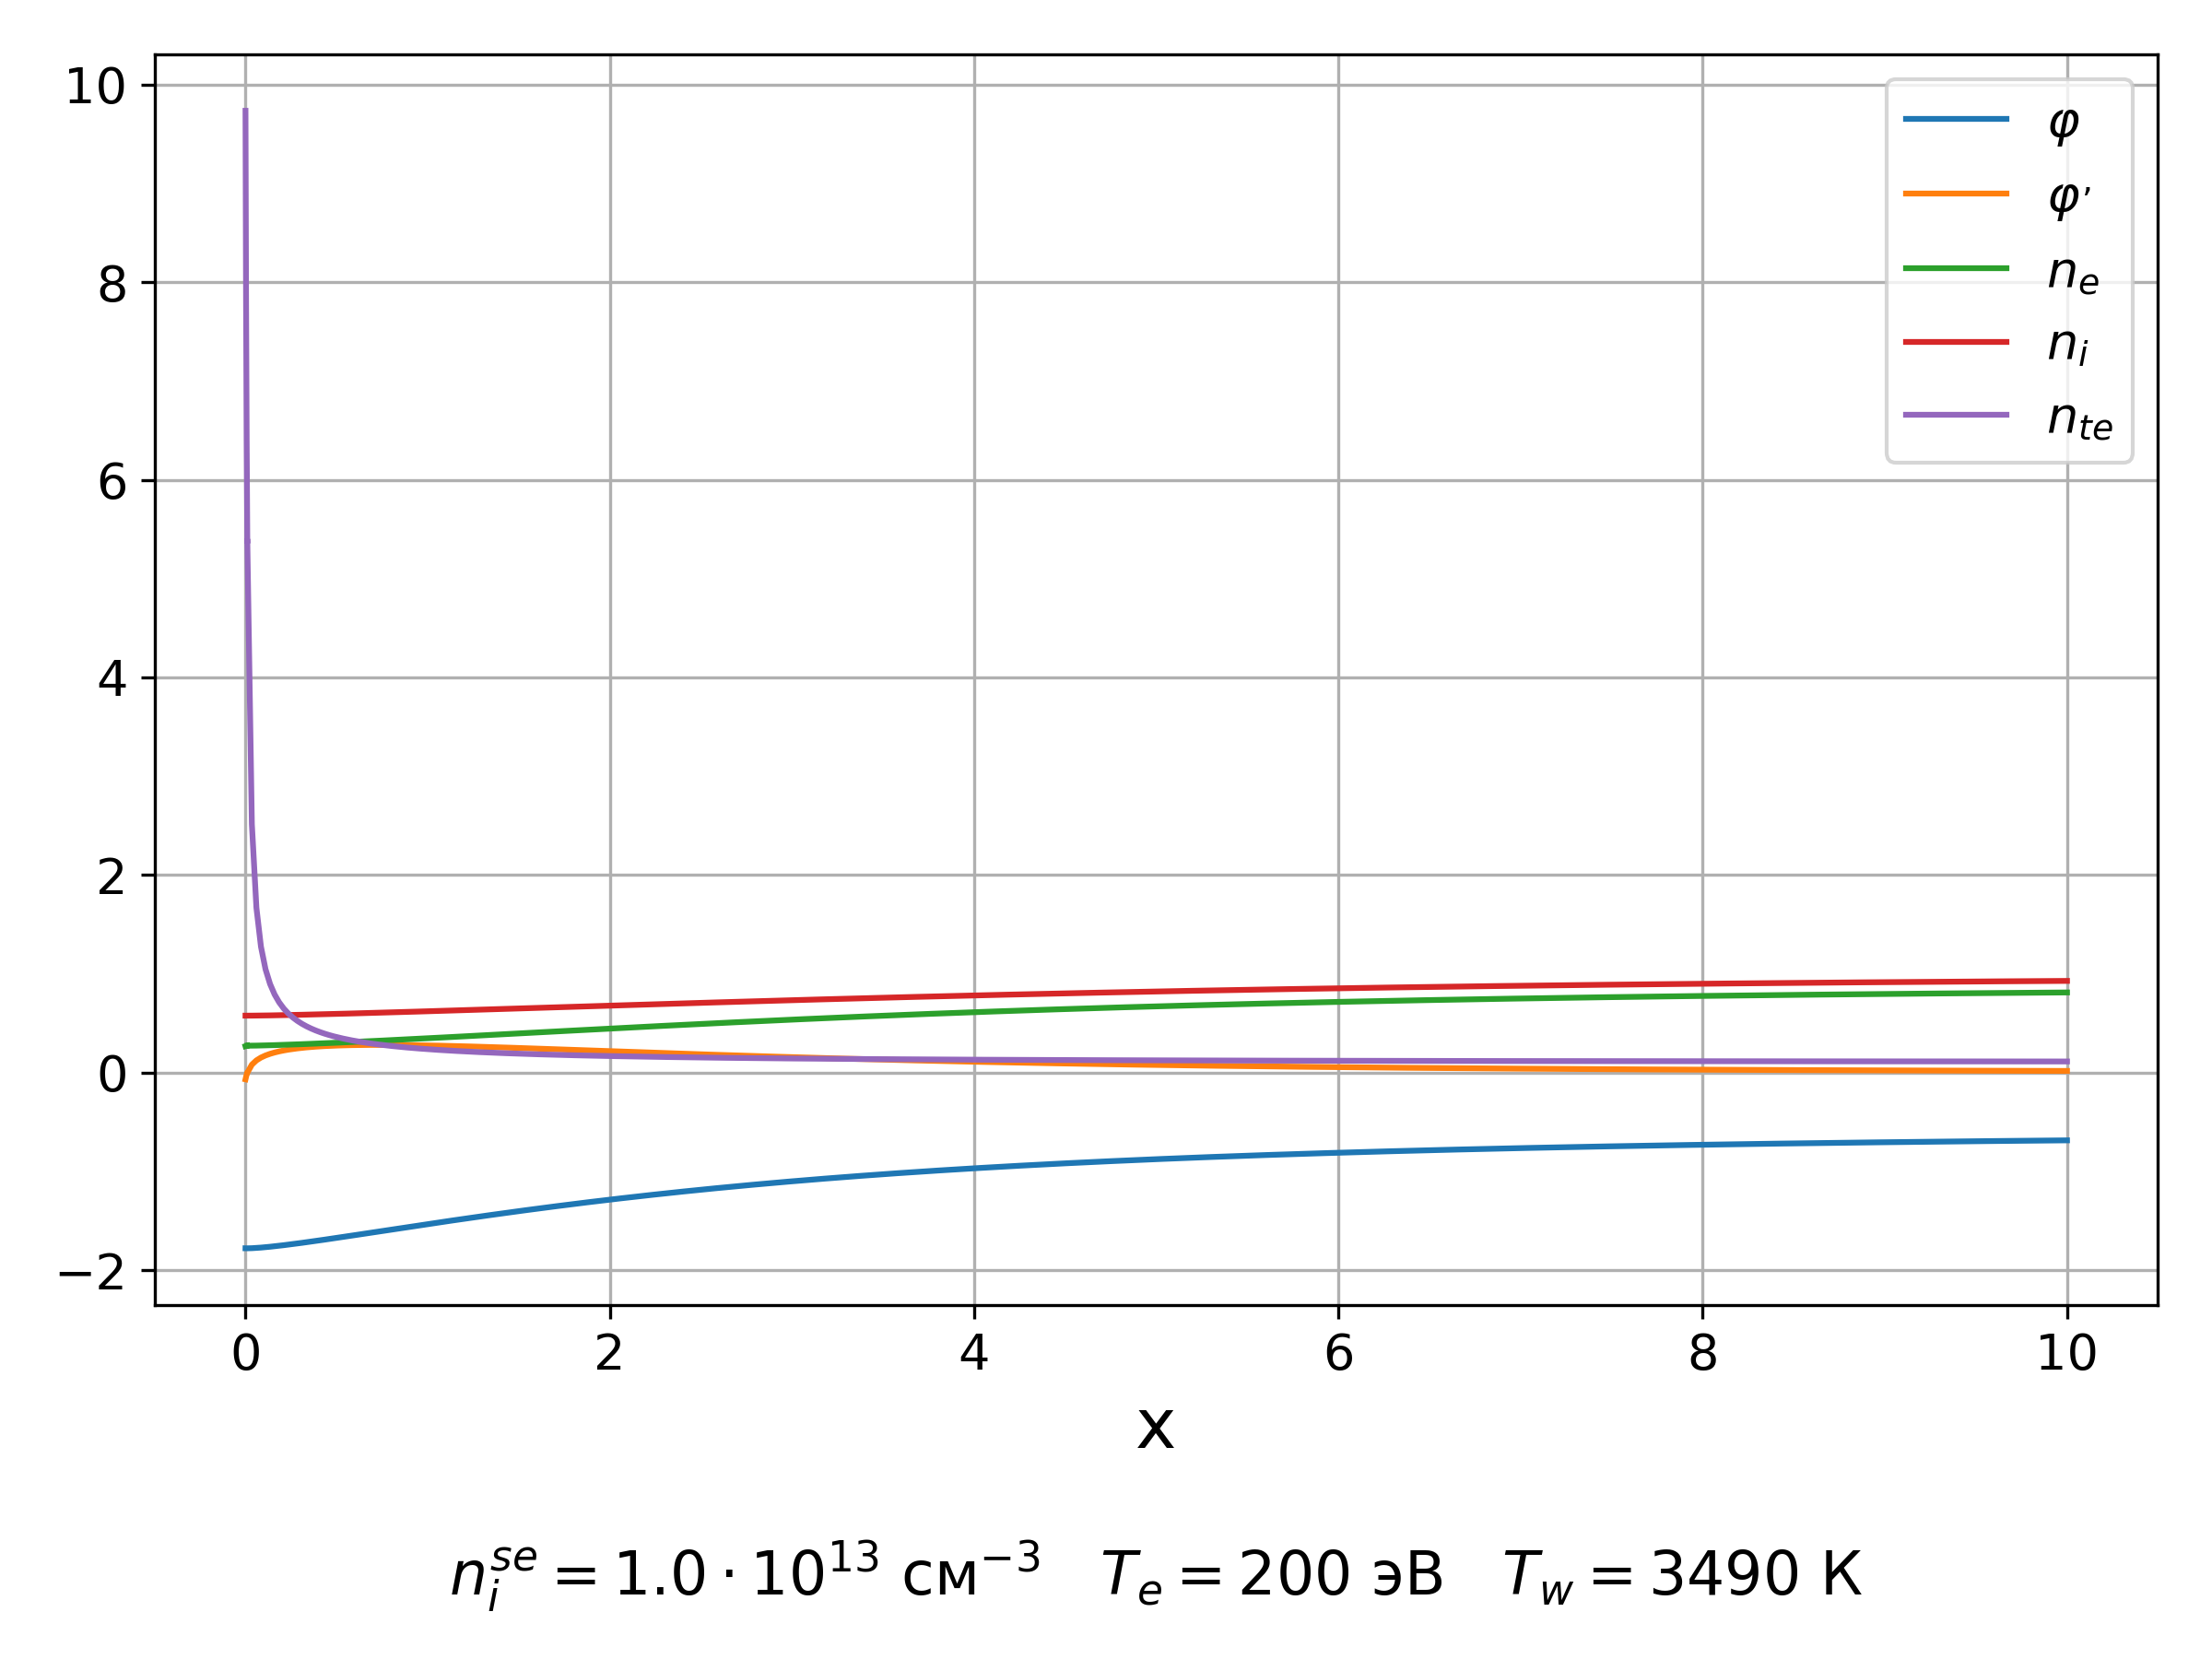
\includegraphics[width=0.7\linewidth]{material/plot_Te=200eV_nse=1.0e13.png}
    \caption[]{В области между поверхностью плитки и входом в дебаевский слой}
	  \end{subfigure}%
    \hfill
	\begin{subfigure}{\textwidth}
	  \centering
        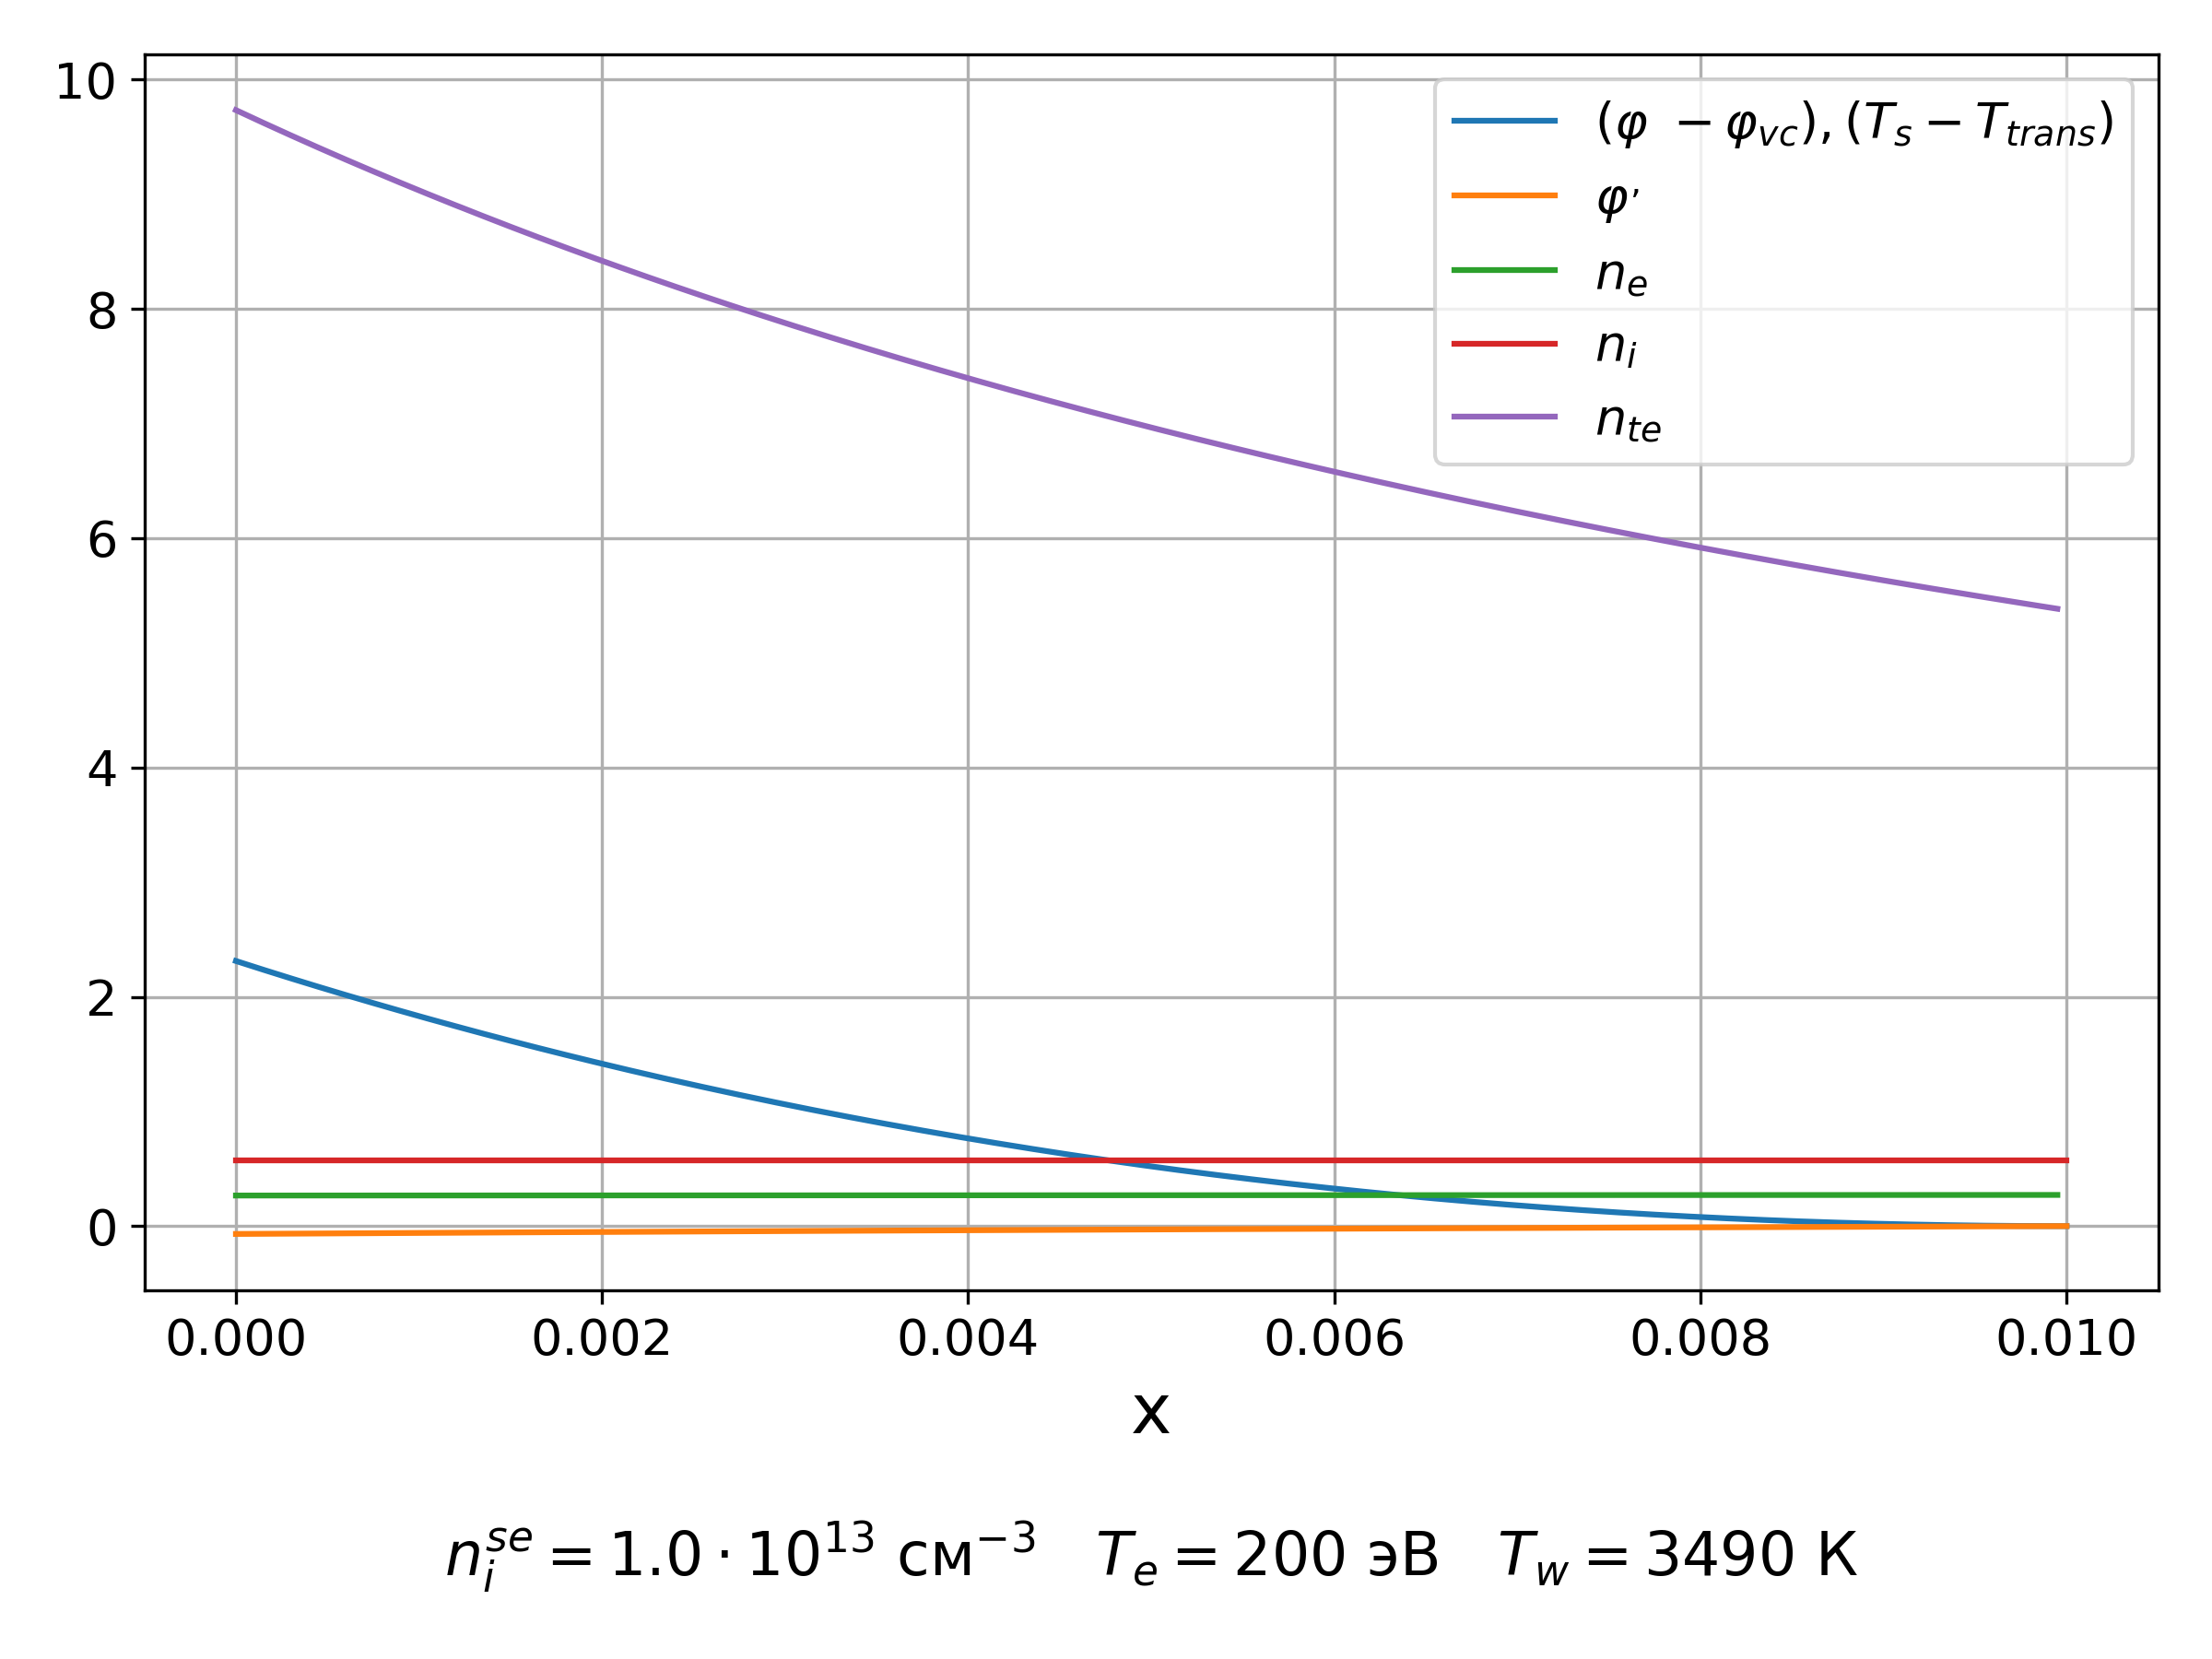
\includegraphics[width=0.7\linewidth]{material/plot_alpha_Te=200eV_nse=1.0e13.png}
    \caption[]{В области между поверхностью плитки и виртуальным катодом}
	\end{subfigure}%
    \caption[]{Графики решений уравнения Пуассона в режиме объёмного экранирования зарядом}
	\label{pic::Model::results::Poisson_Te-200eV_ne-1e13cm^-3}
\end{figure}
\clearpage

\section{Учет теплопроводности в материале}

Перенос тепла в материале стенки на достаточно малых временах может быть описан одномерной задачей:
\begin{subequations}
    \begin{align}
        \partial_t u &= a^2 \partial^2_x u\\
        \left(\partial_x u\right)(x = d) &= \varkappa q_{plasma}\\
        u(x = 0) &= T_0 \\
        u(t = 0) &= T_0 \\
        0 < x &< d \\
        t &> 0
    \end{align}
    \label{eq::heatcond_problem_decl}
\end{subequations}
$a^2 = \cfrac{\varkappa}{C_p\rho}$ --- коэффициент температуропроводности, $\varkappa$ --- коэффициент теплопроводности
Для вольфрама при $T = 1000$ К, параметры имеют значения:
\begin{subequations}
    \begin{align*}
        \varkappa = 118\text{ Вт/(м$\cdot$К)}\\
        \rho = 19.1\cdot 10^3\text{ кг/м$^3$}\\
        C_p = 144.5\text{ Дж/(кг$\cdot$ К)}
    \end{align*}
\end{subequations}

ПЛМ является выбросом плазмы из основного объёма реактора. Ввиду отличной проводимости \hl{сколько?порядка проводимости стали}, 
она ``вмораживает`` магнитные линии, осциллирующие с частотой порядка $10^8$ Гц~\cite{kirk2006evolution}. Осцилляции 
магнитного поля приводят к осцилляции электростатического потенциала. Принимая, что скорость ионов сохраняется, 
эти осцилляции могут представлены как осцилляции потенциала $V_f$.

Задача~\eqref{eq::heatcond_problem_decl} может быть решена методом линий\hl{цитата}.

Проводимость дебаевского слоя может быть описана значением импеданса~\cite{myra2015radio}:
\begin{equation}
    \cfrac{1}{z} = \cfrac{\langle JV\rangle}{\langle V^2\rangle} - \cfrac{i\omega\langle J\dot{V}\rangle}{\langle \dot{V}^2\rangle}
\end{equation}

\begin{figure}[H]
	\centering
	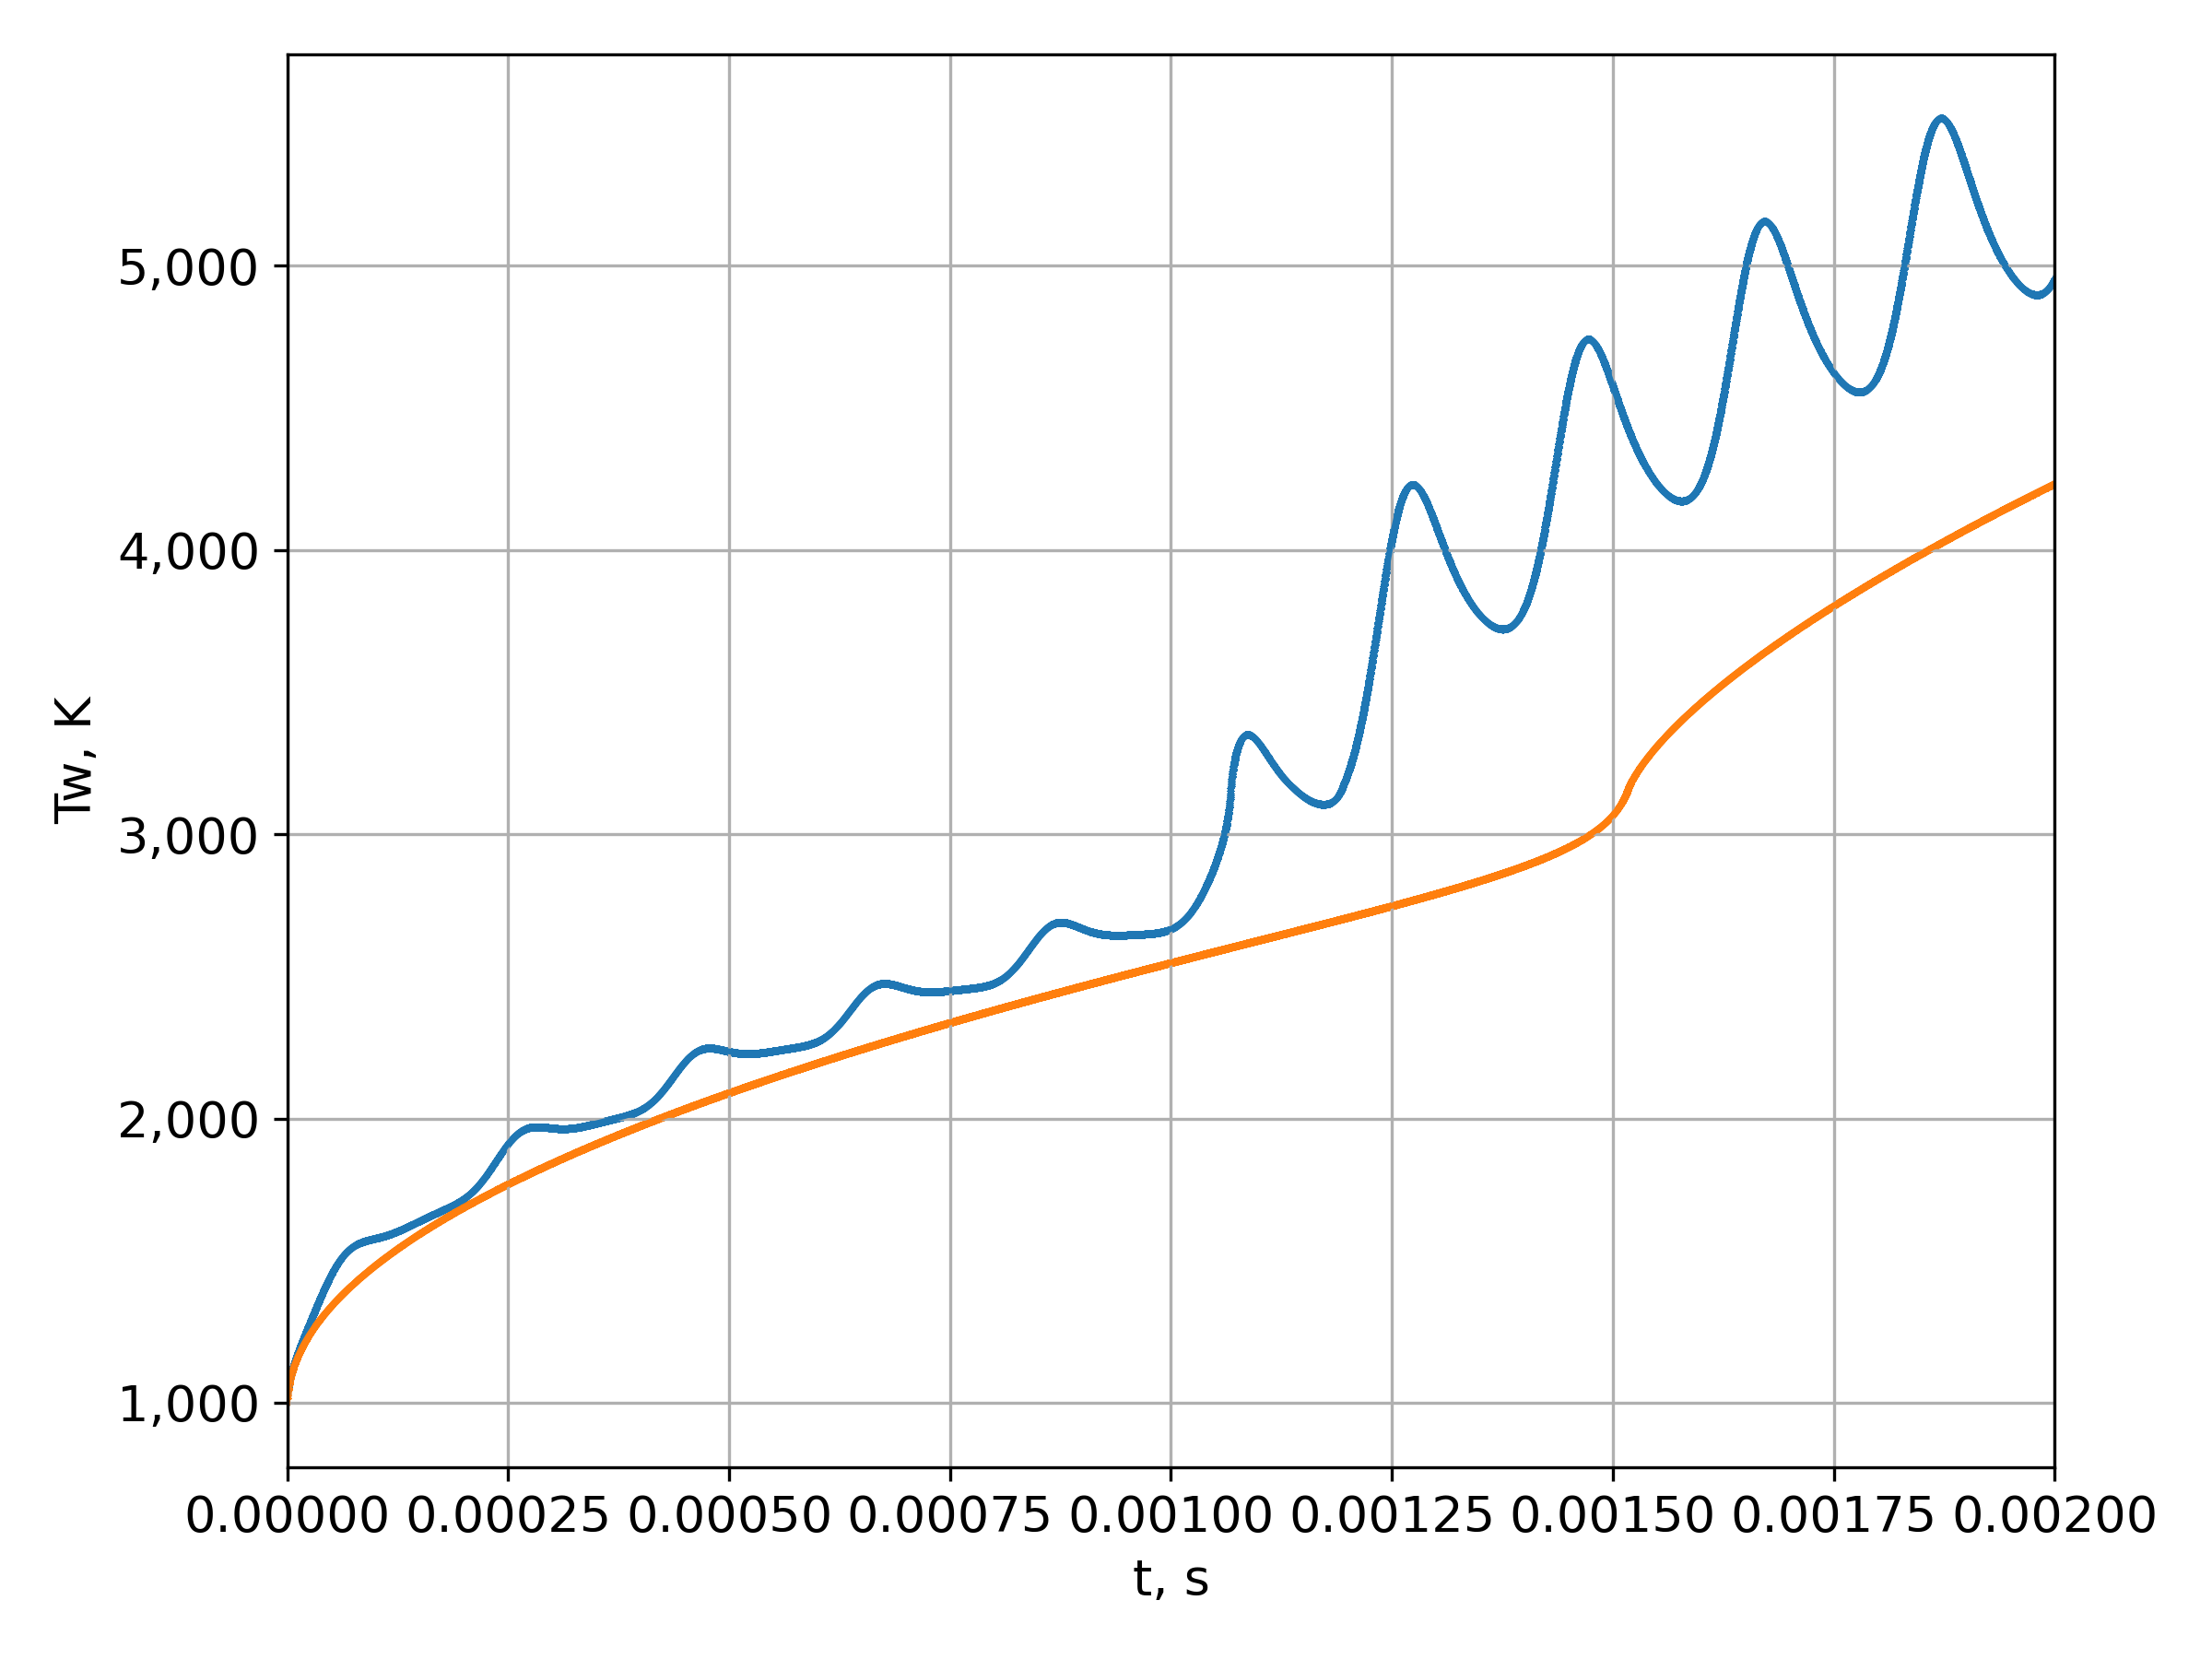
\includegraphics[width=0.7\linewidth]{material/omega10amp1.0/temperature_plot.png}
    \caption[]{Эволюция температуры поверхности плитки $T_s$}
    \label{pic::heatcond::omega10amp1.0::temperature_plot}
\end{figure}

\begin{figure}[H]
	\centering
	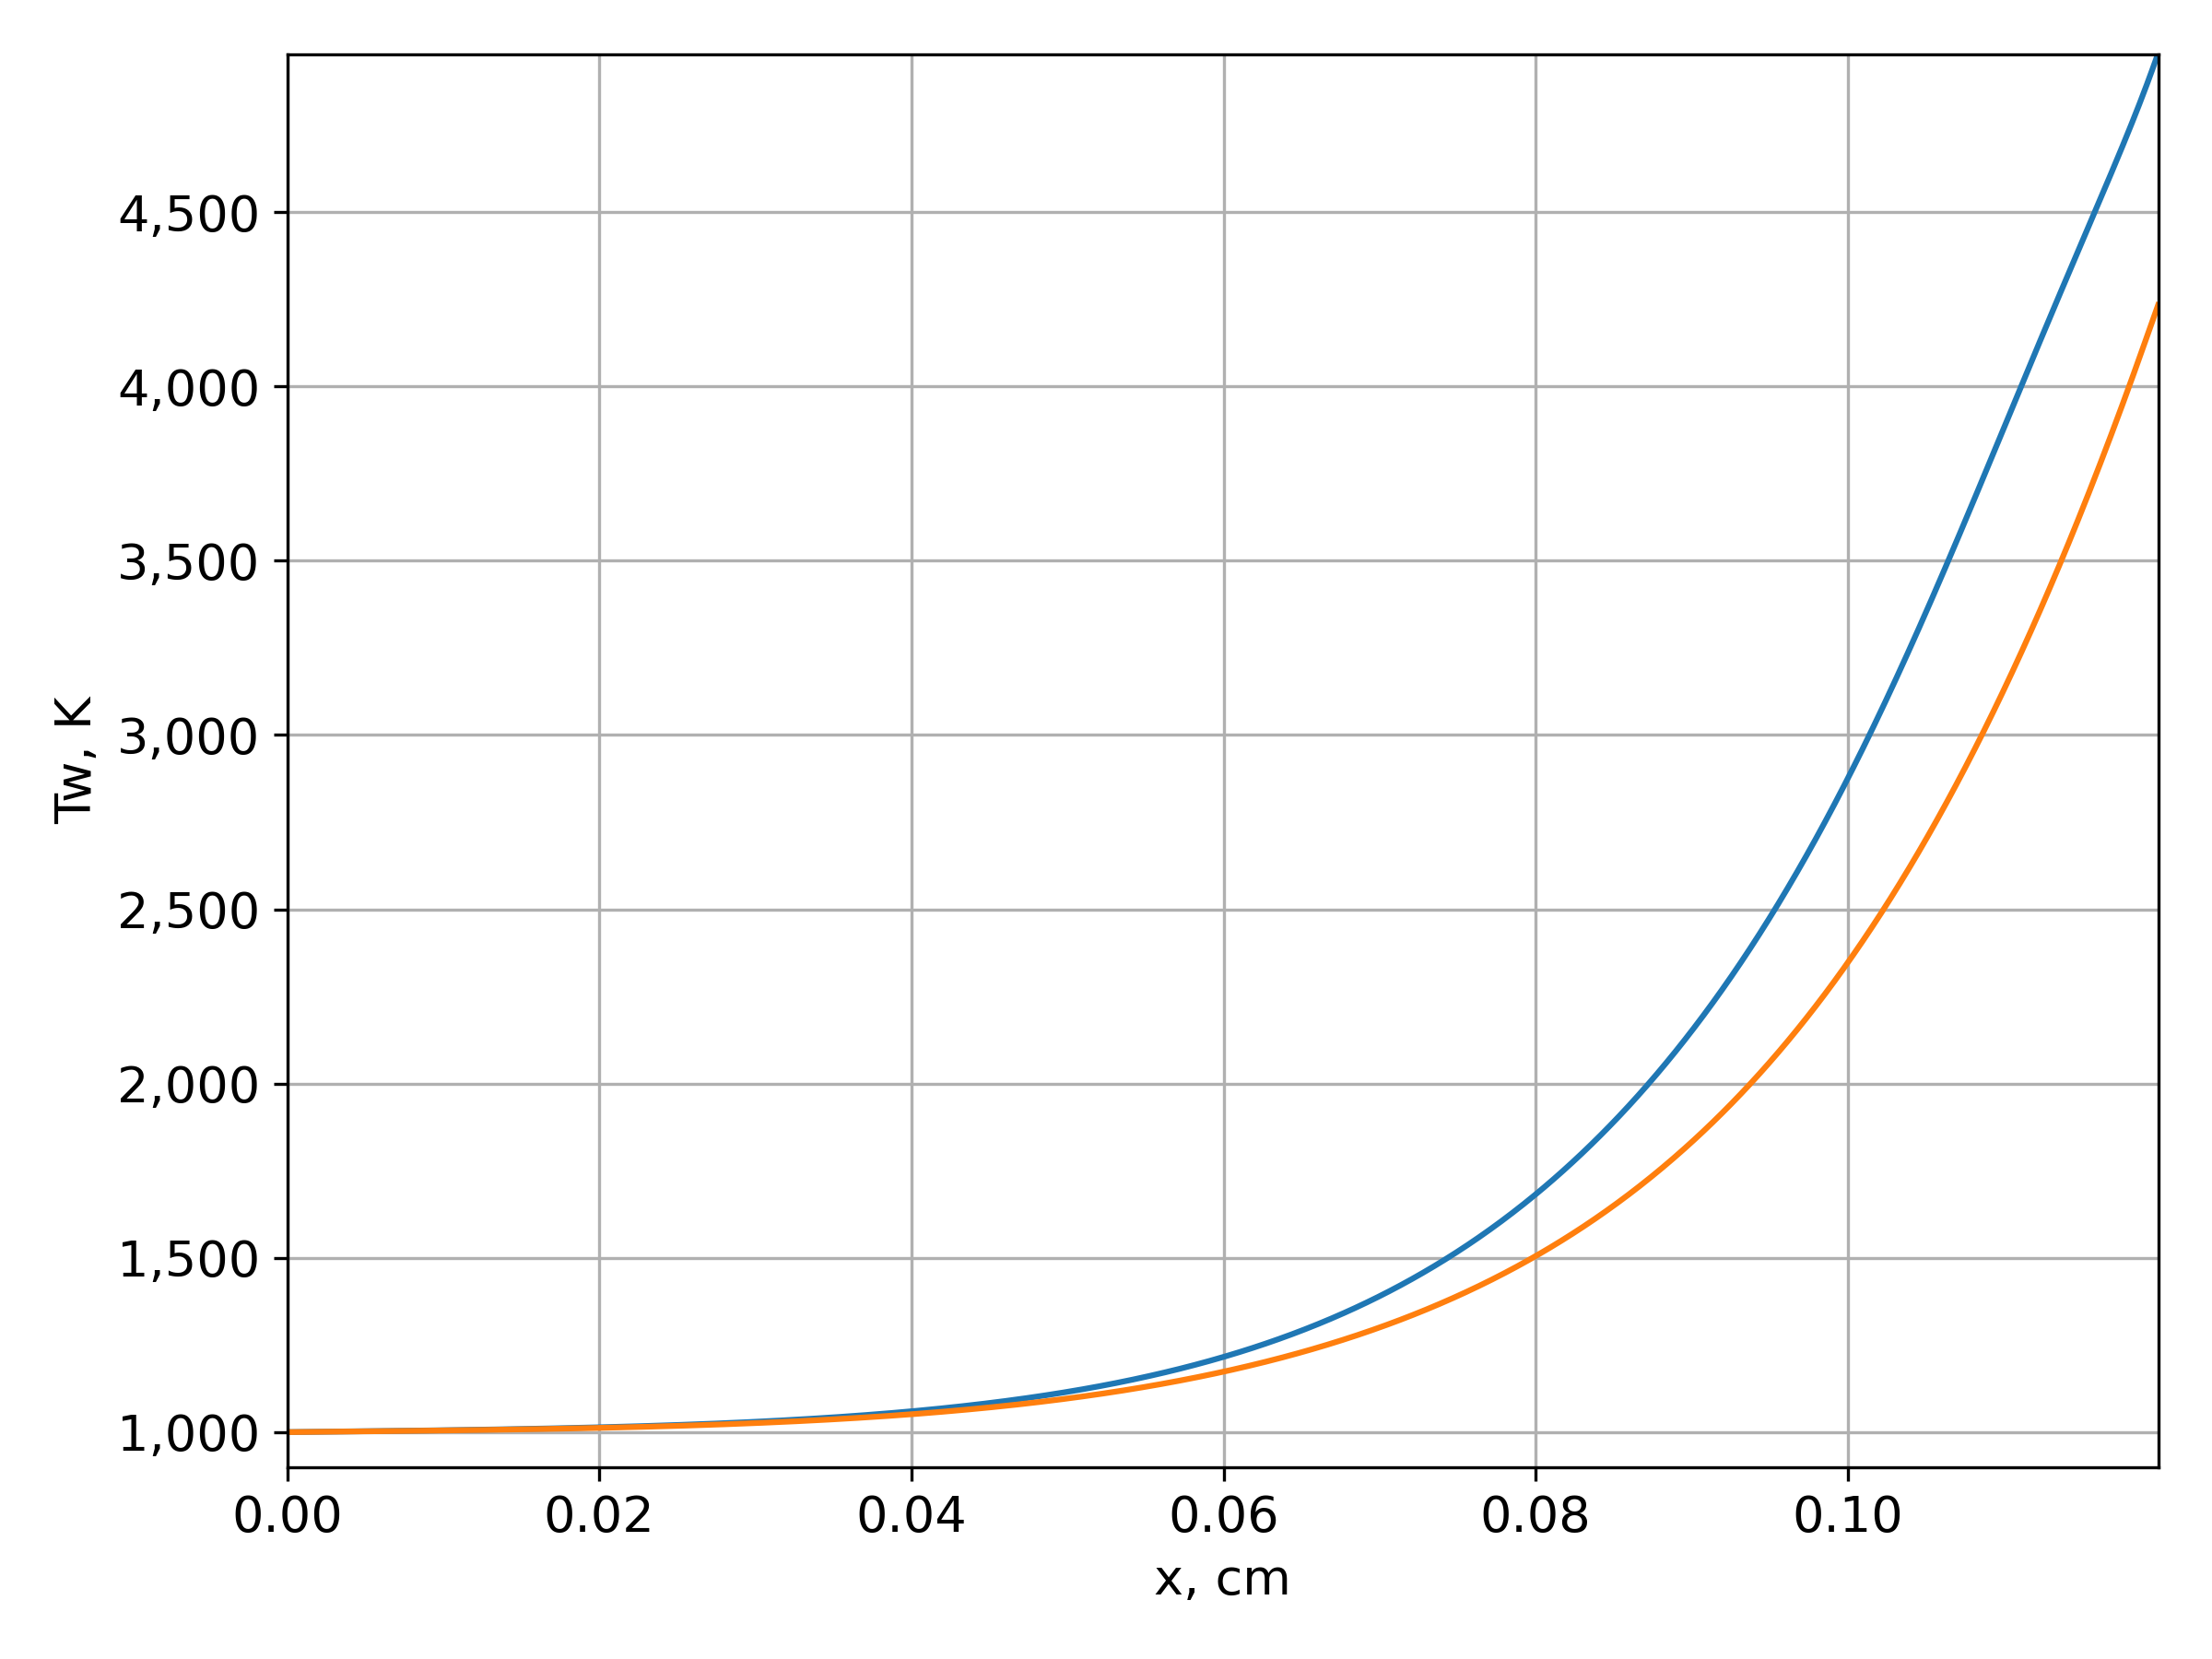
\includegraphics[width=0.7\linewidth]{material/omega10amp1.0/temperature_distribution_plot.png}
    \caption[]{Профиль температуры в плитке}
    \label{pic::heatcond::omega10amp1.0::temperature_distribution_plot}
\end{figure}
\begin{figure}[H]
	\centering
	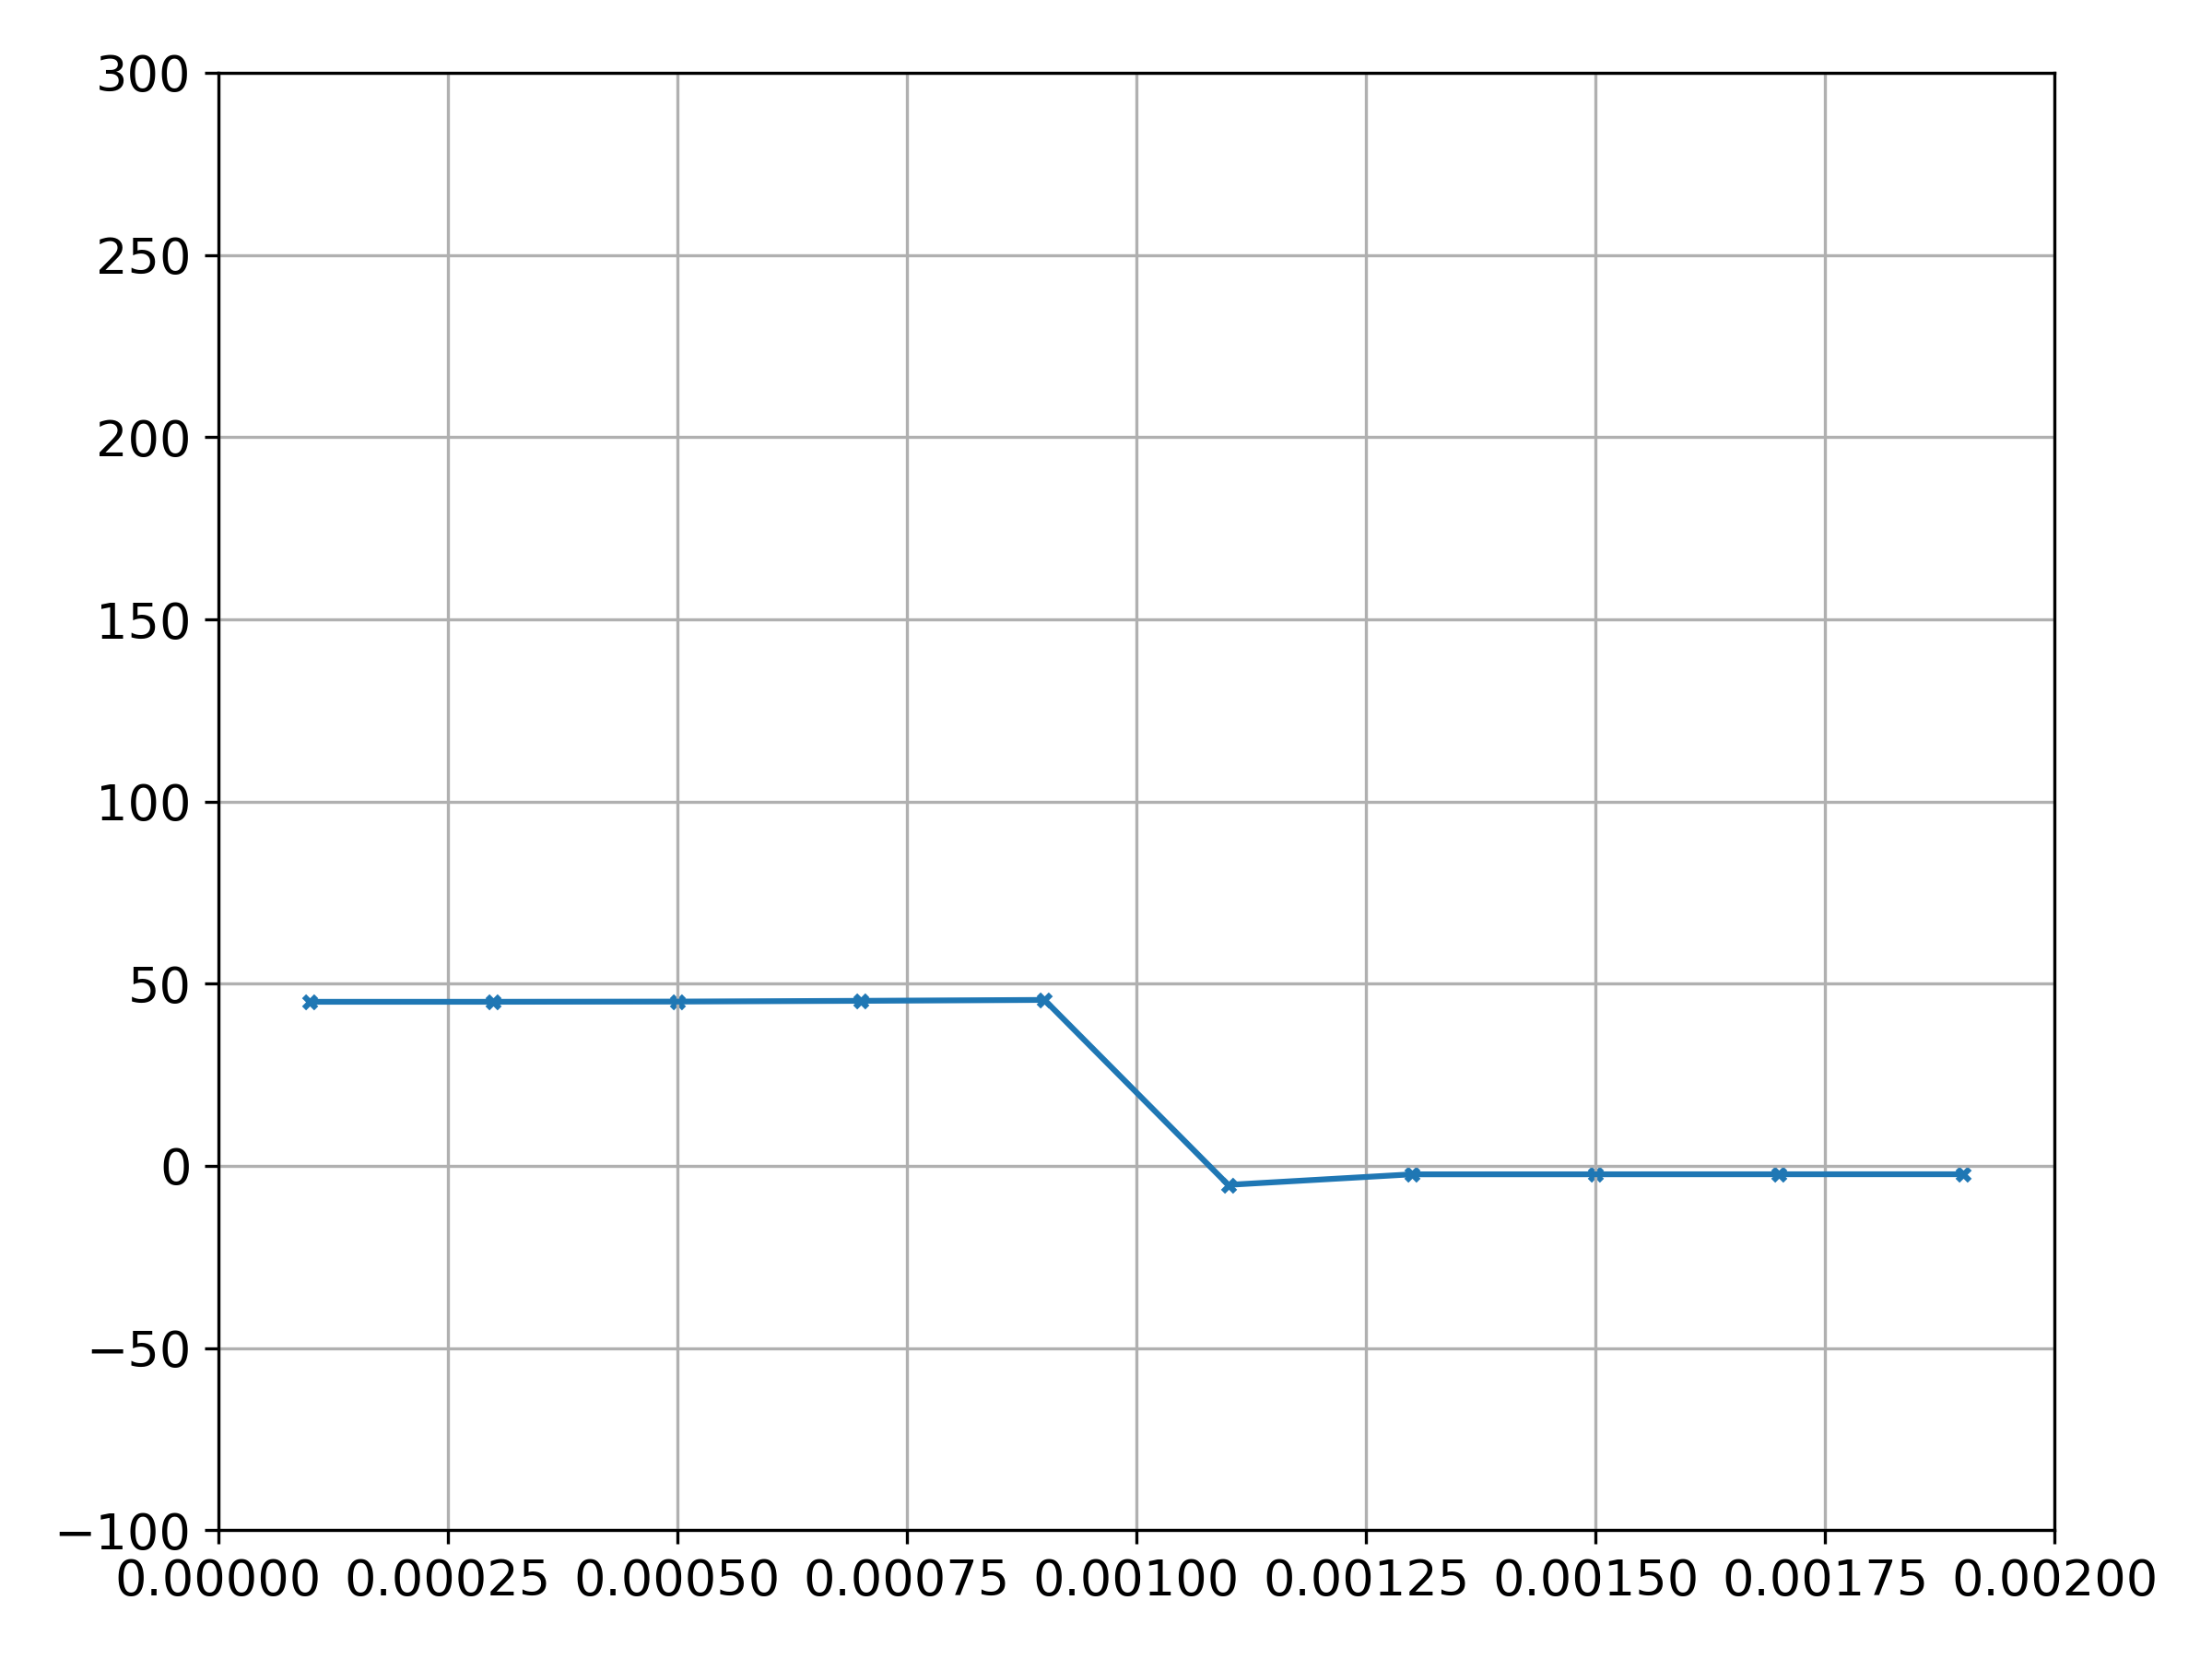
\includegraphics[width=0.7\linewidth]{material/z_plot.png}
    \caption[]{Эволюция резистивной части импеданса $z$ }
    \label{pic::heatcond::omega10amp1.0::z_plot}
\end{figure}

\clearpage
\bibliographystyle{siamurl}
\bibliography{mybib}
\end{document}